\documentclass{article}

\usepackage[utf8]{inputenc}
\usepackage{amsfonts}
\usepackage{amsmath}
\usepackage{amsthm}
\usepackage{blindtext}
\usepackage{graphicx}
\usepackage{natbib}
\usepackage{amssymb}

\newtheorem{theorem}{Theorem}
\newtheorem{lemma}{Lemma}
\newtheorem{corollary}{Corollary}
\newtheorem{conjecture}{Conjecture}
\newtheorem{proposition}{Proposition}
\theoremstyle{definition}
\newtheorem{definition}{Definition}
\newtheorem{remark}{Remark}


\title{Hammond's Project and Simple Random Graphs}
\author{by Alan Hammond, Benjamin Lemkin, Emma Lynch, Milo Moses, Samuel Packman}
\begin{document}
\maketitle

\newcommand{\lcm}{\mathrm{lcm}}


\tableofcontents
\newcommand{\R}{\mathbb{R}}
\newcommand{\Z}{\mathbb{Z}}
\newcommand{\N}{\mathbb{N}}
\newcommand{\C}{\mathbb{C}}
\newcommand{\class}{\mathcal{C}}
\newcommand{\E}{\mathbb{E}_{B}}
\newcommand{\Esup}{\mathbb{E}^{\mathrm{sup}}_{n\in\mathbb{N}}}
\newcommand{\rad}{\mathrm{rad}}

\addcontentsline{toc}{section}{}

\section{Introduction}

In this project, the authors seek to understand the behavior of Simple Random Bridge (SRBs), and more specfically how they behave under addition. An SRG of size $N$ is a function $B:\Z/N\Z\to\Z$ such that $B(0)=0$ and $B(x+1)-B(x)=\pm 1$ for all $x\in \Z/N\Z$.

\begin{figure}[h]
\caption{An Example of a SRB}
\centering
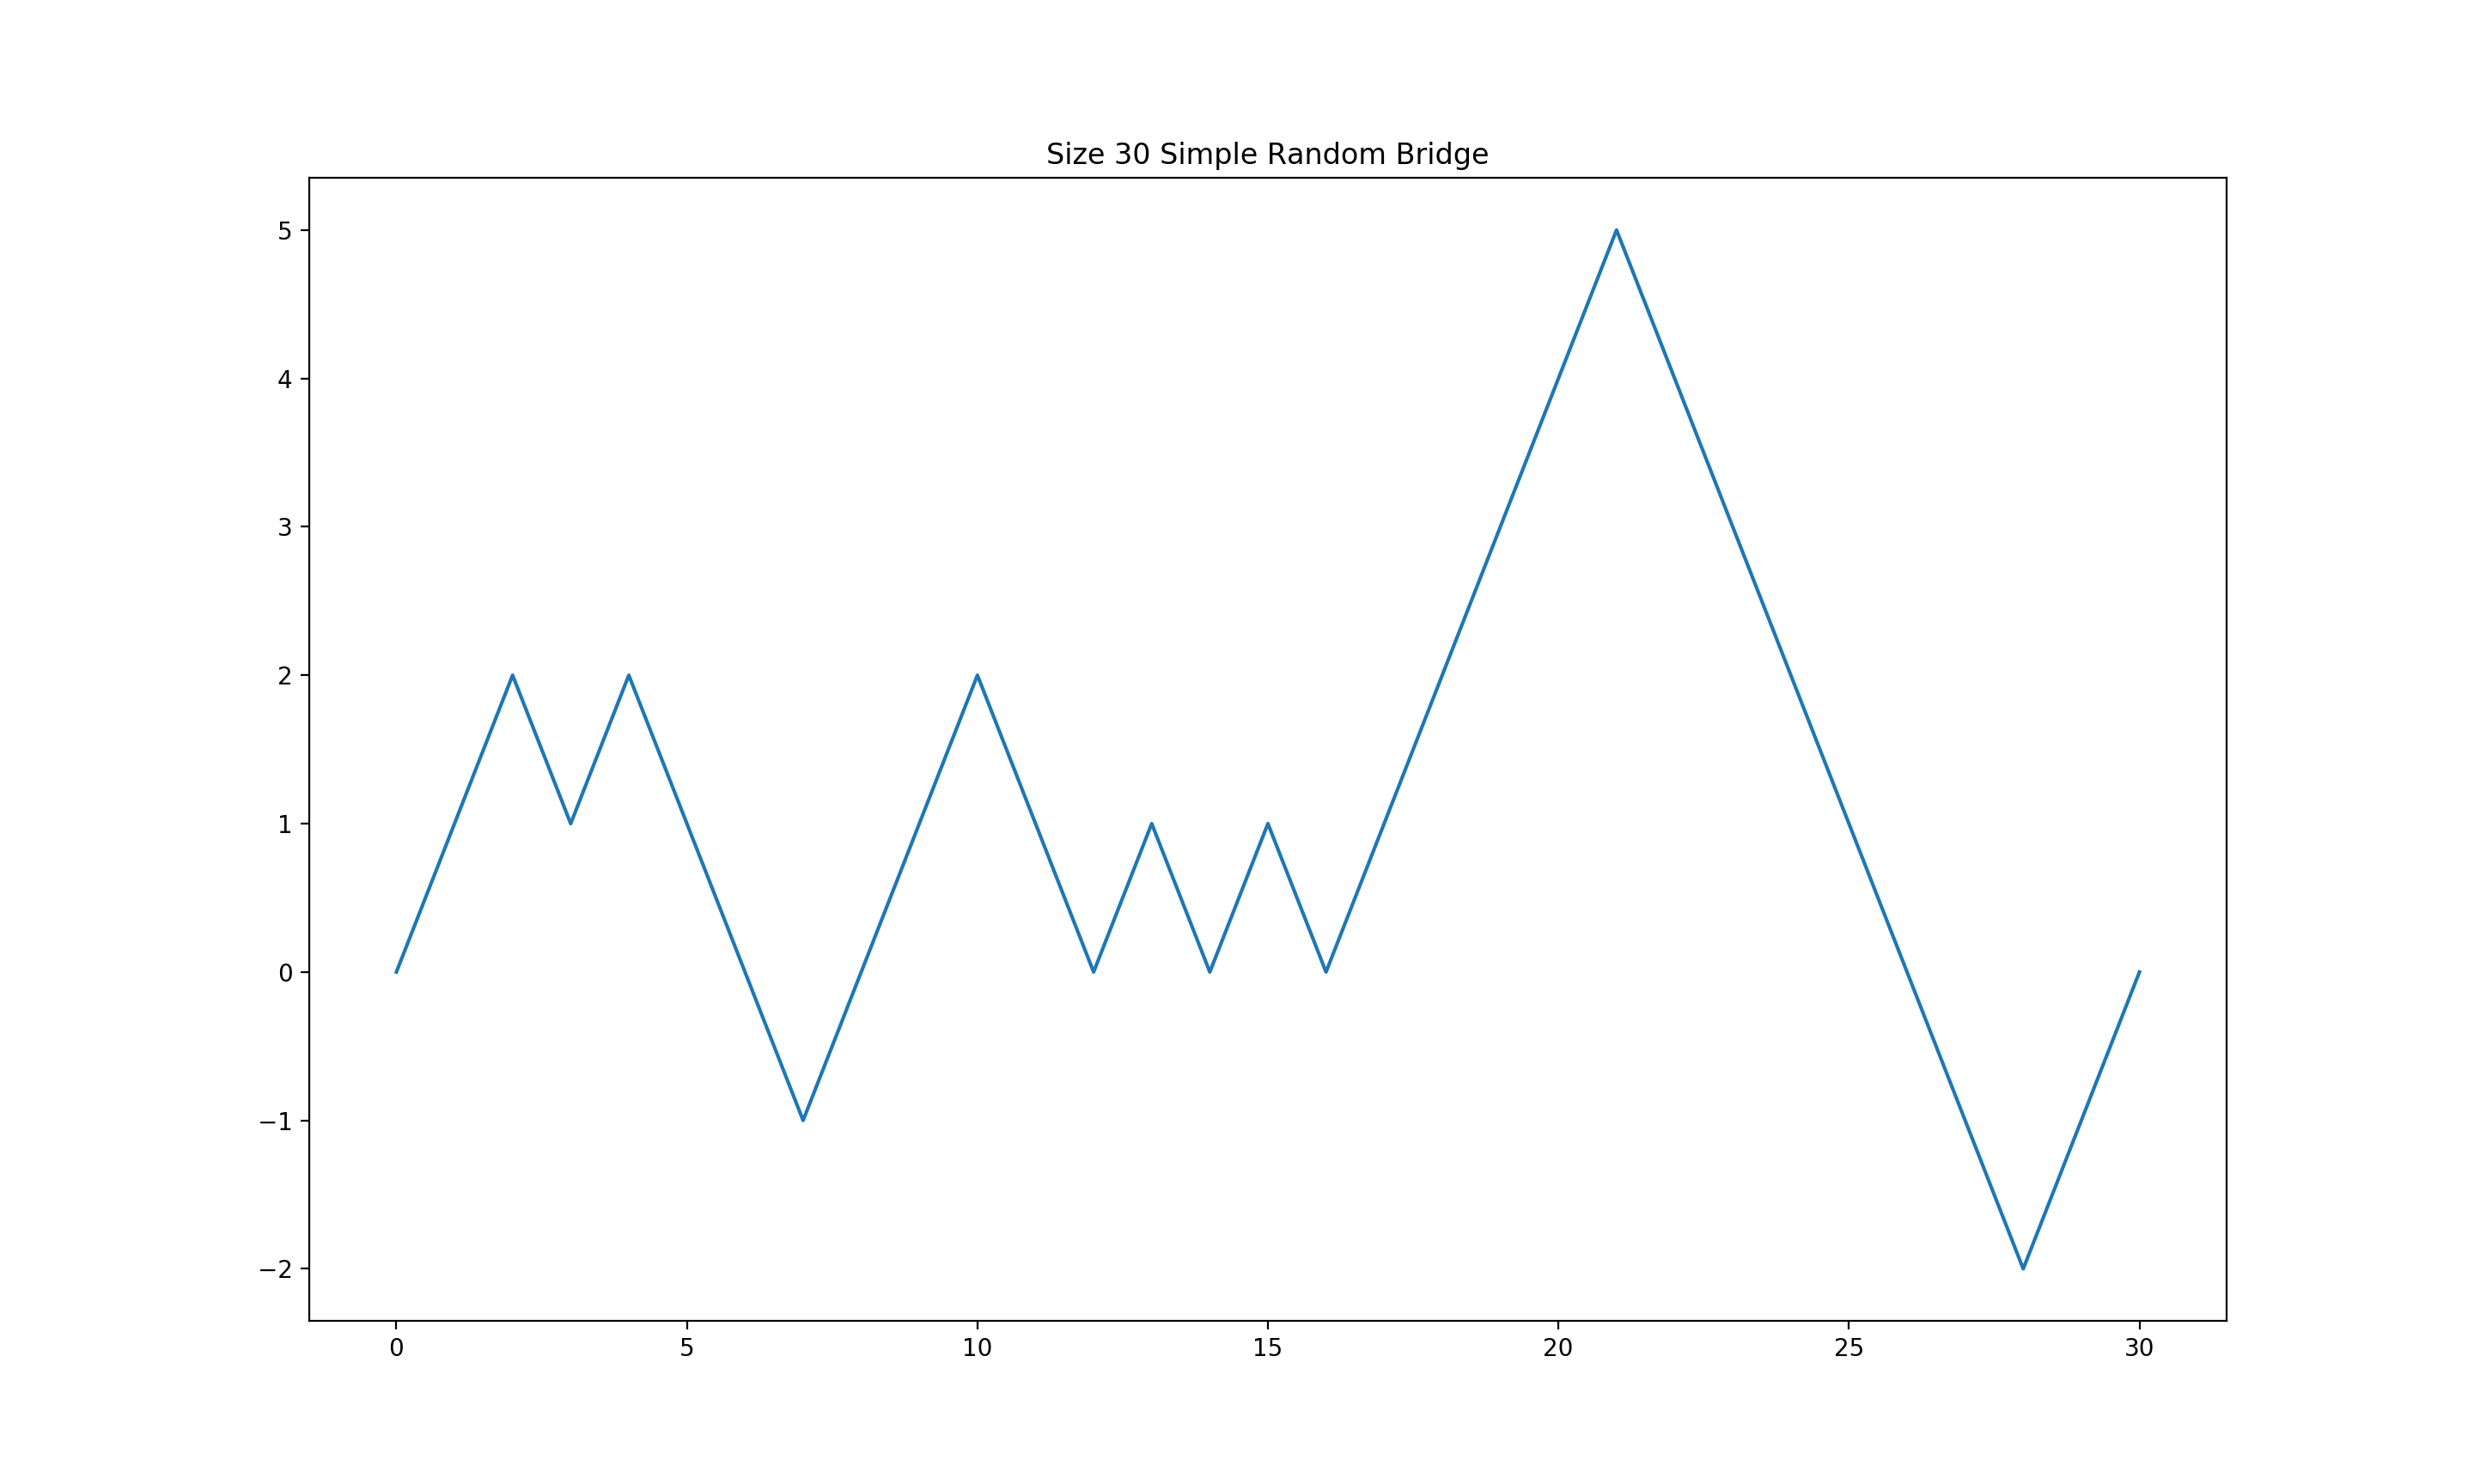
\includegraphics[width=\textwidth]{Figure_1}
\end{figure}

We say that a value $i\in \Z/N\Z$ is $\mathit{down}$ in $B$ if $B(i)<\min(B(i-1),B(i+1))$.

If $B_1$ and $B_2$ are size $N$ bridges, then we say that the $\mathit{minimal \,\,points}$ of $B_1$ under $B_2$ are those values $i\in \Z/N\Z$ such that $B_1(i)-B_2(i)=\min_{j}\left(B_1(j)-B_2(j)\right)$. If $0$ is not minimal then we define the $\mathit{addition}$ of $B_2$ to $B_1$ as

\begin{equation*}
\tilde{B_1}(i)=\begin{cases} B_1(i)+2 & i \,\,\mathrm{minimal\,\, under\,\,}B_2 \\
B_1(i)& \mathrm{otherwise}
\end{cases}
\end{equation*}

If $0$ is minimal, then we define

\begin{equation*}
\tilde{B_1}(i)=\begin{cases} B_1(i)-2 & i \,\,\mathrm{not\,\,minimal\,\,under\,\,}B_2 \\
B_1(i)& \mathrm{otherwise}
\end{cases}
\end{equation*}

It is clear that in both cases $\tilde{B_1}$ is once again an SRB. We note the interpretation of addition as putting $B_2$ below $B_1$ (as graphs) and sliding $B_2$ up until it just touches $B_1$, at which point every down intersection point is flipped up. In the case that $0$ is minimal, everything is then rescaled down so that $\tilde{B_1}(0)=0$.

The main interest of this paper is the result of repeated addition of a template bridge $B_1$ to random trial bridges, where in this context random means taken uniformly over the (finite) space of SRBs of size $N$.

\begin{figure}[h!]
\caption{An SRB after repeated addition}
\centering
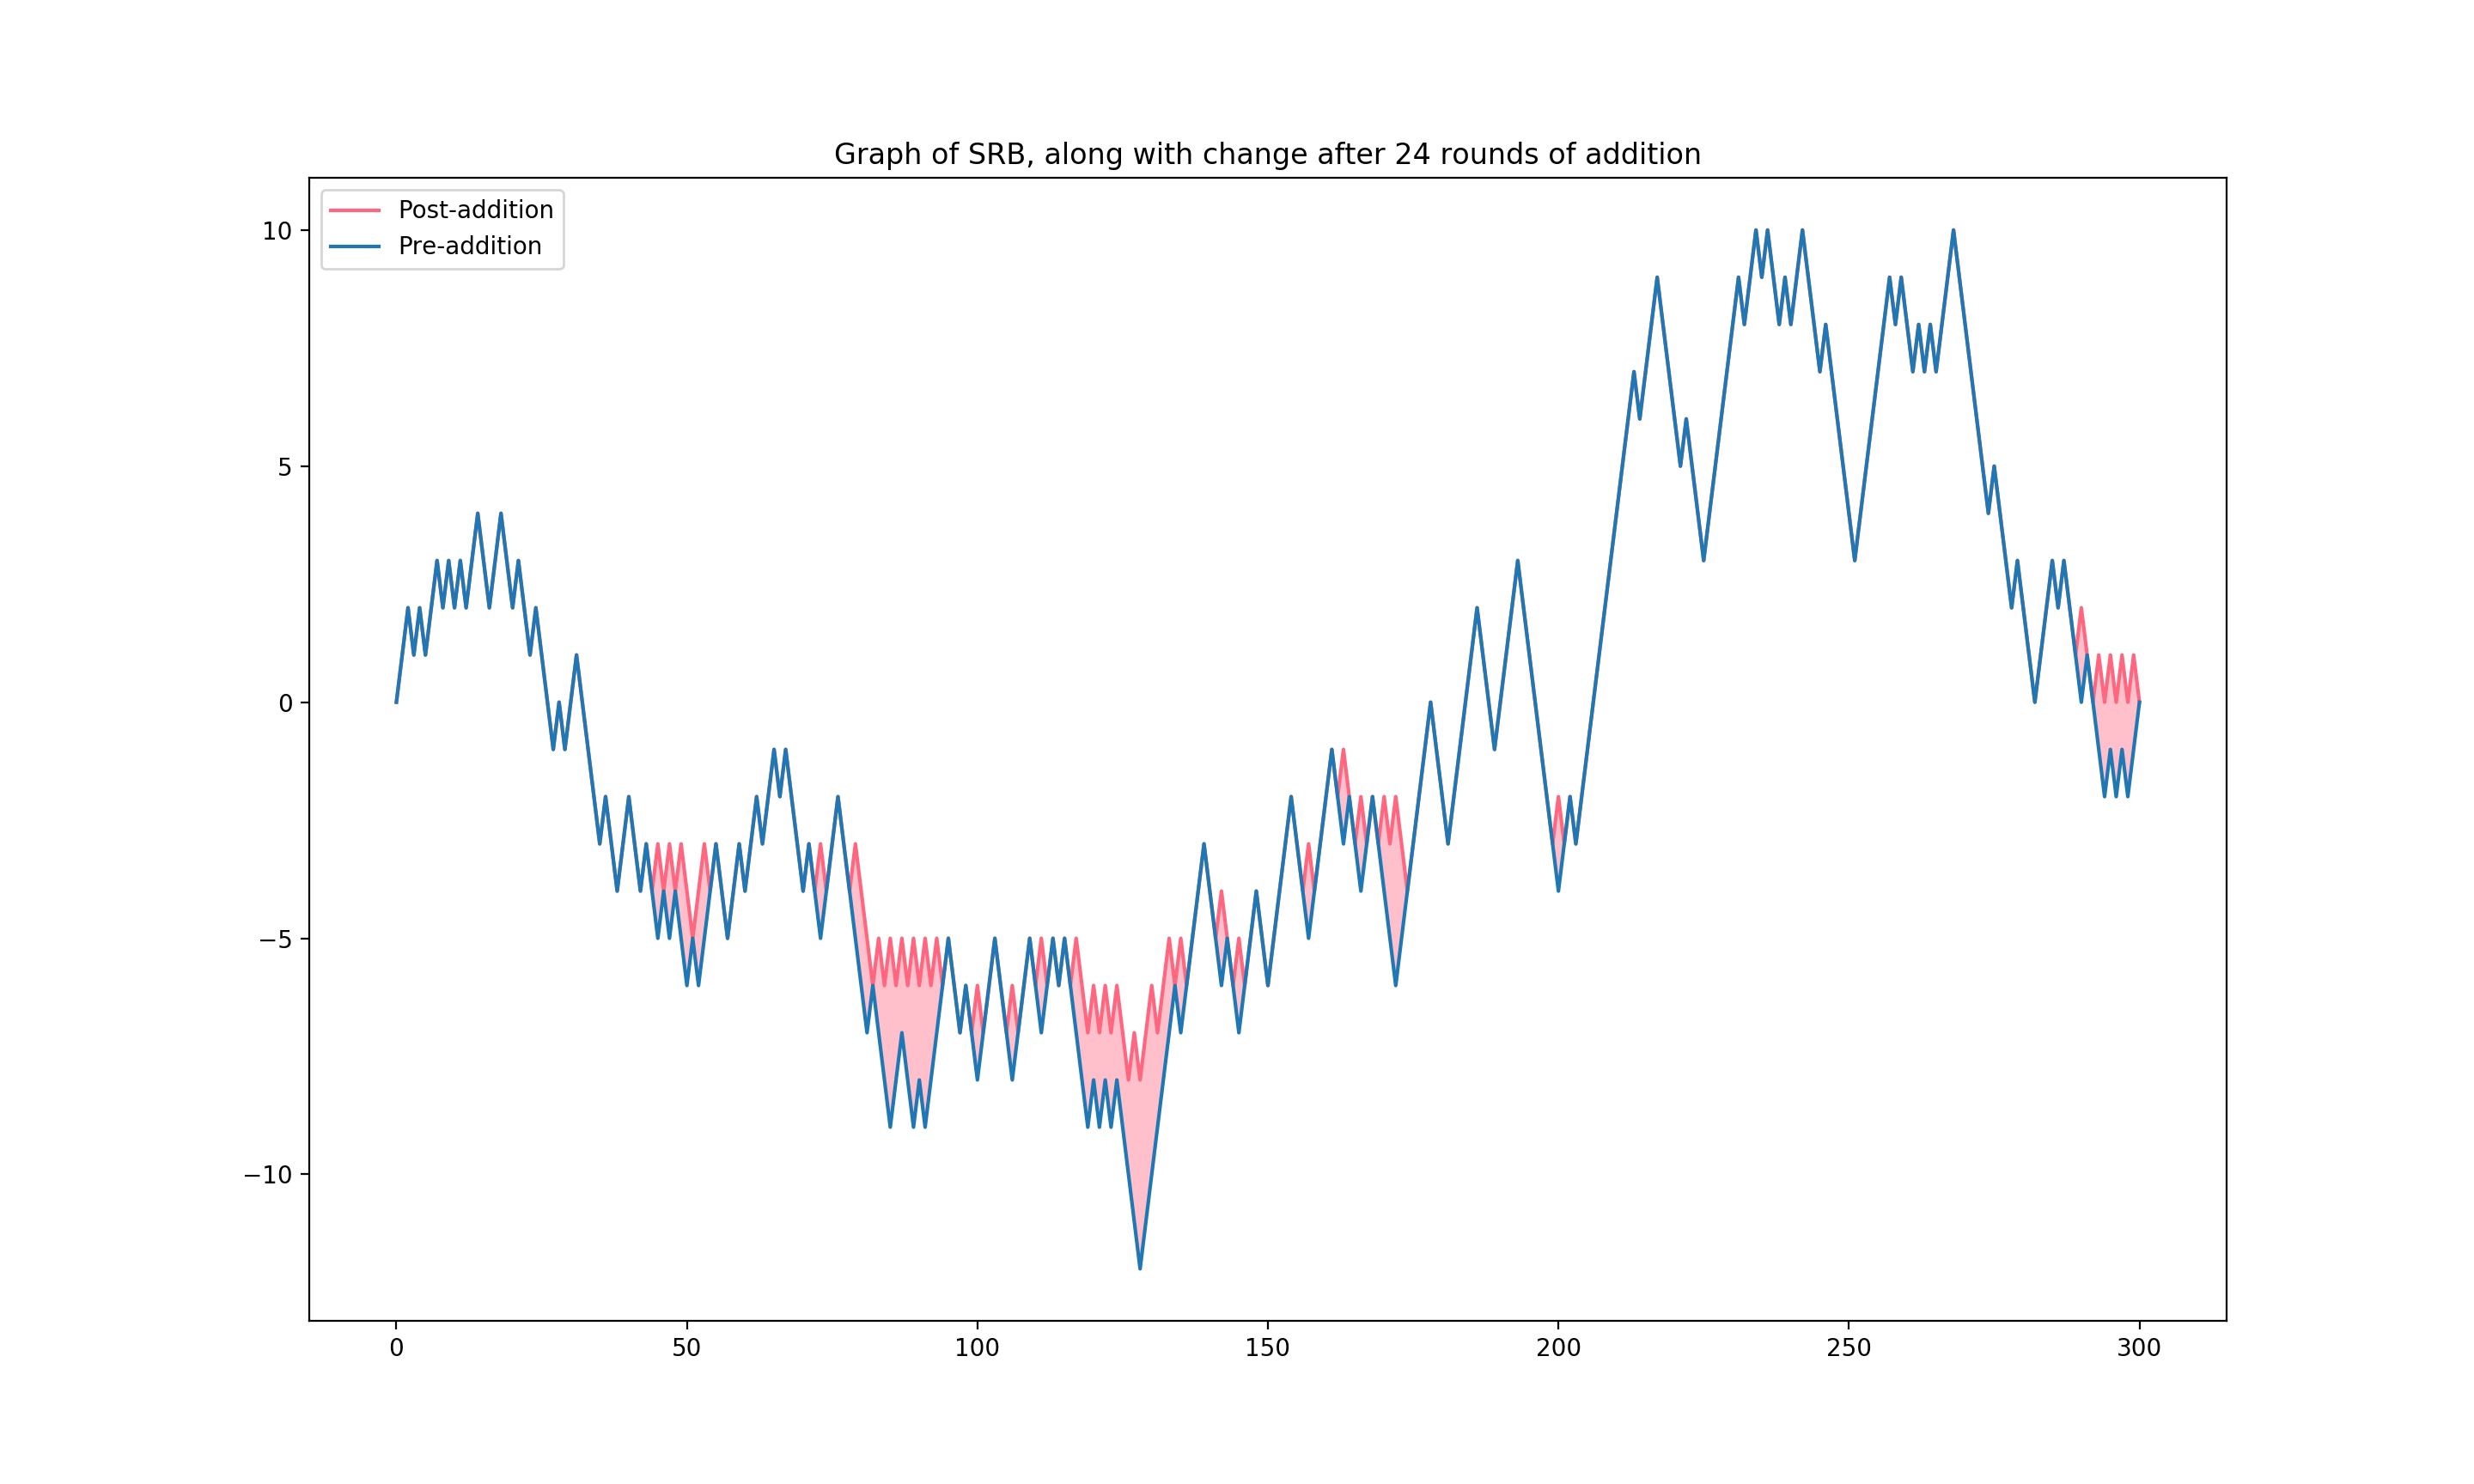
\includegraphics[width=\textwidth]{Figure_2}
\end{figure}

\section{Flattening effect of repeated addition}

One natural phenominon to observe the probability that any given SRB appears after large rounds of repeated addition. A sampling of 100 random SRBs of size 176 before and after 10,000 rounds of repeated addition by random SRBs is shown in Figure 3.

\begin{figure}[h!]
\caption{100 SRBs after repeated addition}
\centering
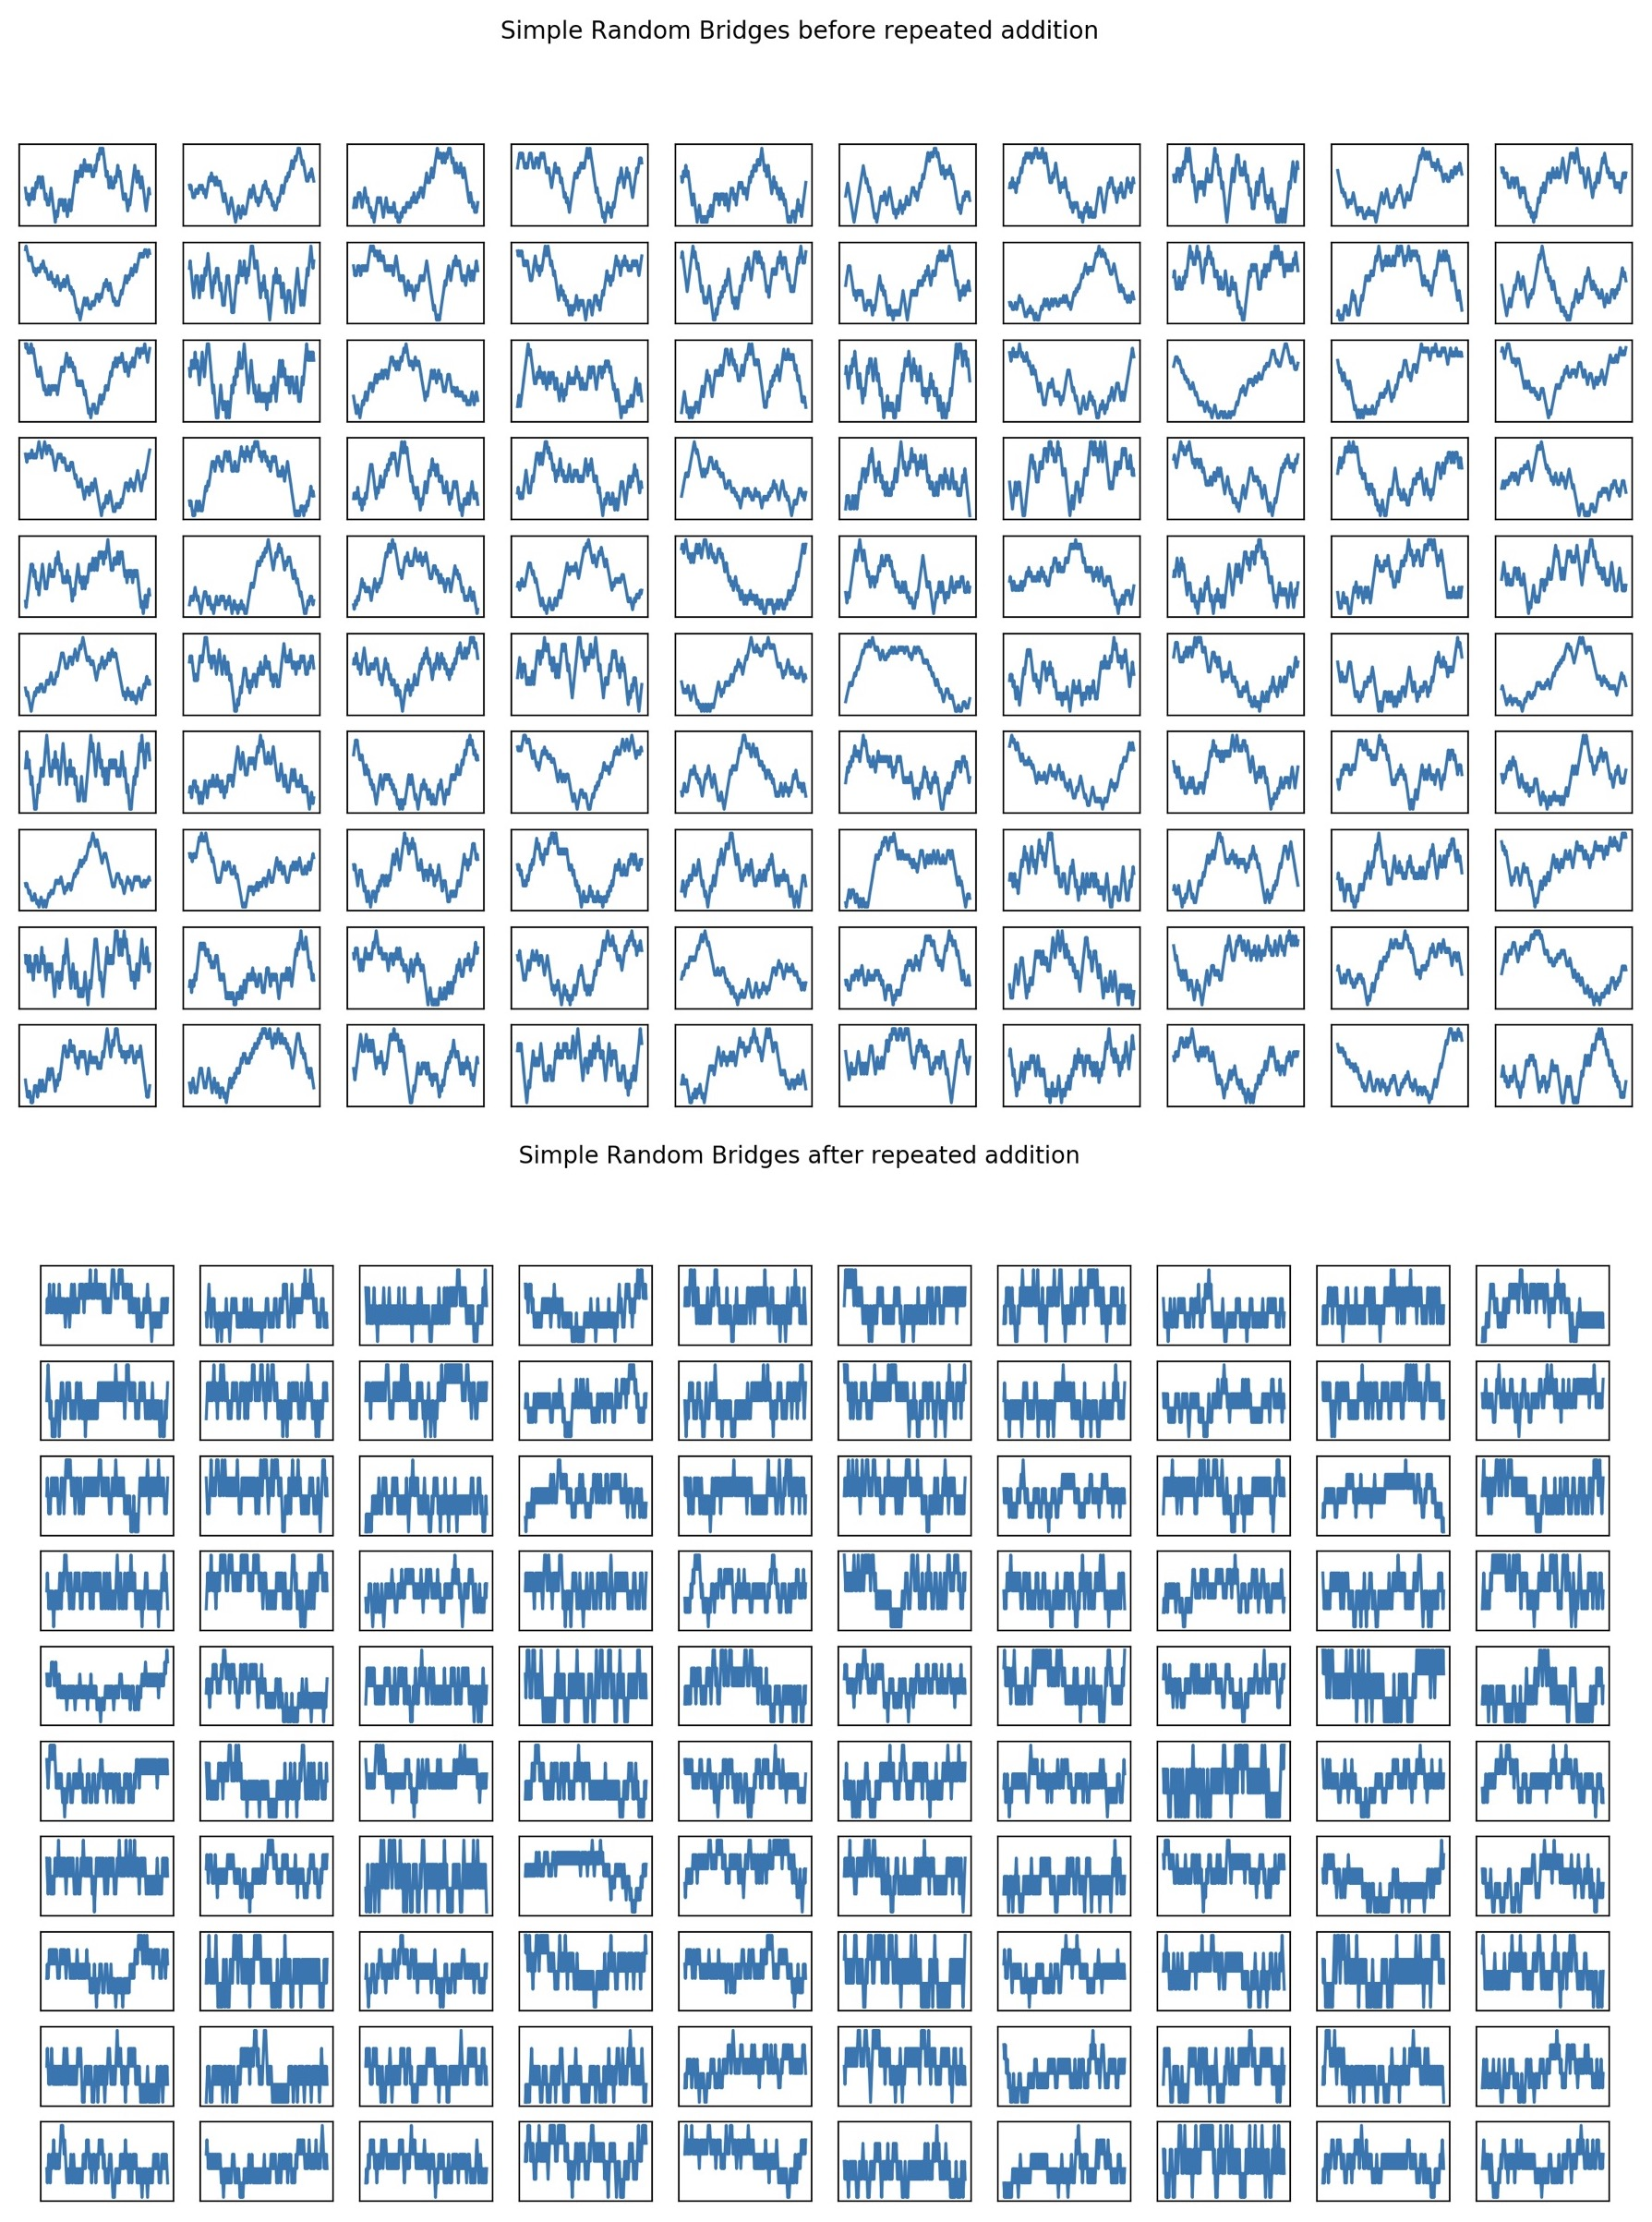
\includegraphics[width=.75\textwidth]{Figure_3}
\end{figure}

Note the the thick bars in the "after repeated addition" group. These show that the values of $B$ are distributed across a very small image. This can be measured in the quantity $s(N):=\E\left[\max_{i}|B(i)|\right]$ where the expected value is taken over all bridges $B$ of size $N$, weigthed according to how likely they are to appear after an arbitrarily large amount of flips from an arbitrary starting bridge. This example demonstrates the fact that, numerically, $s(176)$ seems to be about $2.8$.

Figure 4 shows how the numerically approximated quanity $s(N)$ changes as $N$ varies. Due to the extremely sharp fit of the superimposed logarithm, the following conjecture is clearly motivated:

\begin{conjecture} The value $\lim_{N\to\infty}\frac{s(N)}{\ln(N)}$ converges to a value $0<c<\infty$.
\end{conjecture}

\begin{figure}[h!]
\caption{s(N) versus $N$}
\centering
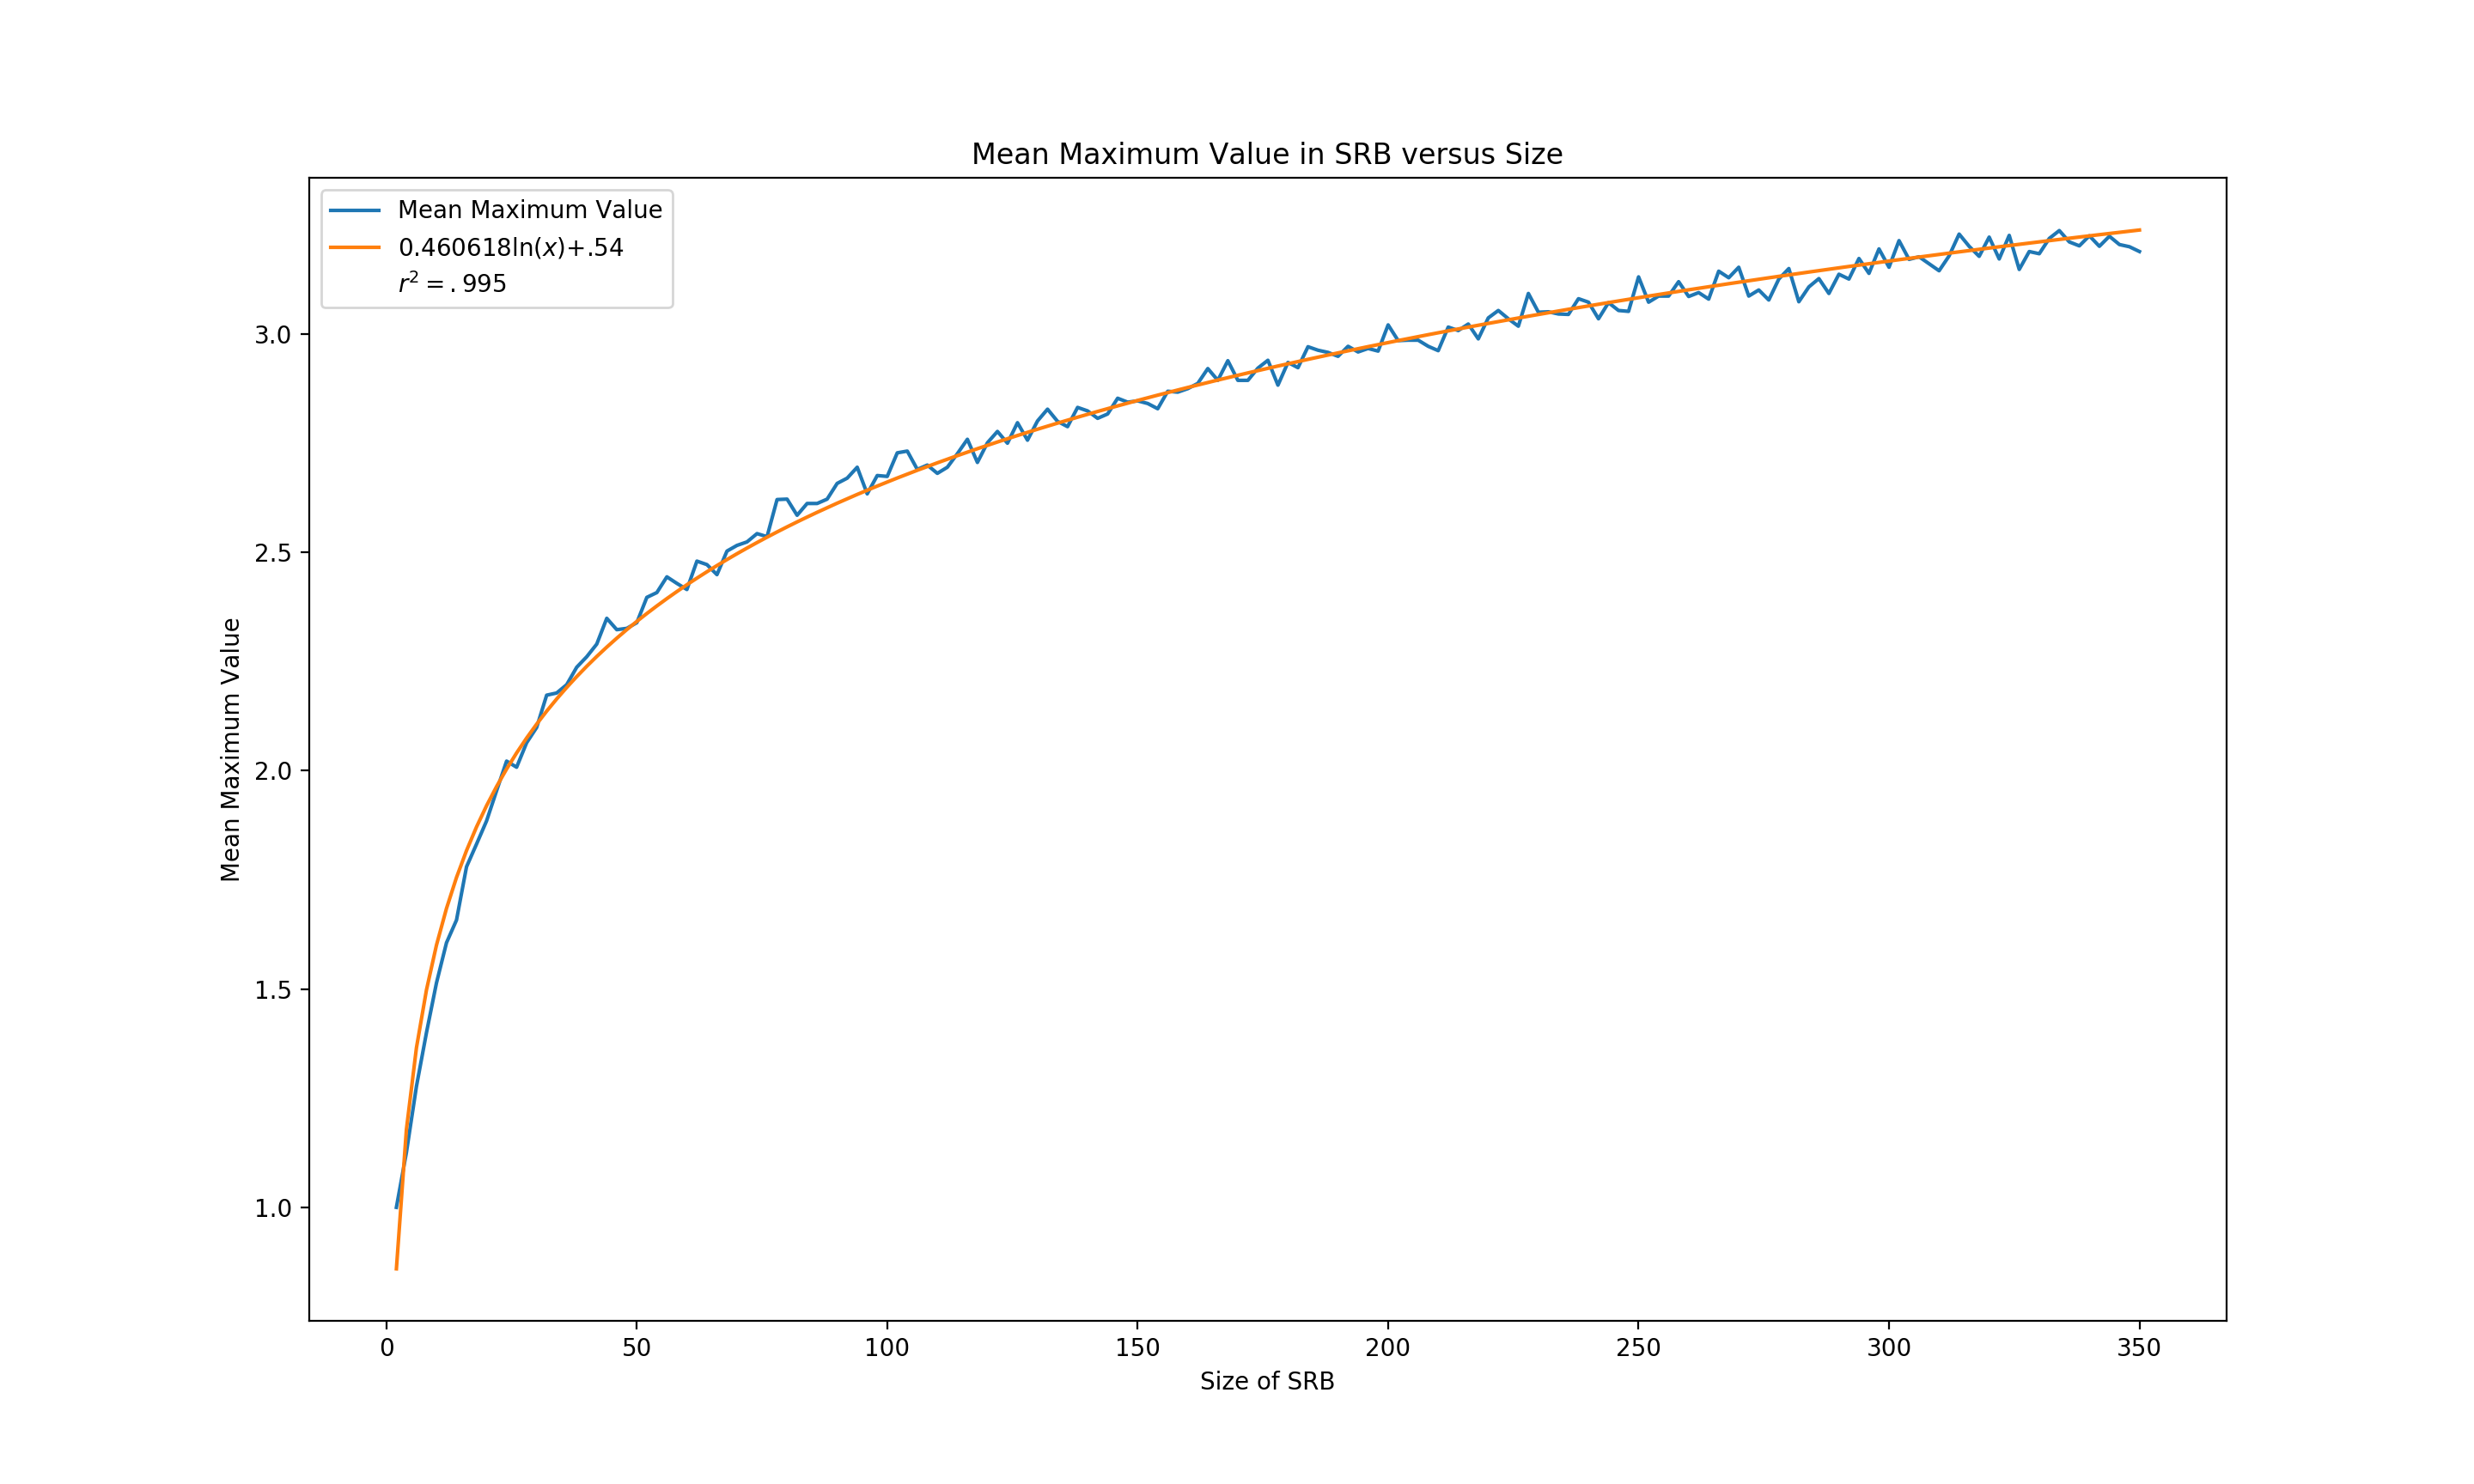
\includegraphics[width=\textwidth]{Figure_4}
\end{figure}


\section{Probability of point specific flips under addition}

One way that one might hope to understand the behavior of SRBs under addition would be to examine the probability that any individual down point is flipped. A specific SRB with its points colored according to the probability that they are flipped is shown in Figure 5. While sharp general results seem hard to come by, there are a few simple statements that one can make about these probabilities.

In the below proposition and throughout, the probability is taken uniformly as $B$ is added with all test bridges $B_0$ of size $N$.

\begin{proposition} Let $B$ be the SRB of size $N$ defined by $B(i):=(i\,\,\mathrm{mod}(2))$, which is well defined as there are no SRBs for which $N$ is odd. It holds that

$$\Pr[0\,\,\mathrm{flips}]=\frac{8(N+1)}{(N+3)(N+4)}$$
\end{proposition}

\begin{proof} By the definition of probability we have that

\begin{equation}
\Pr[0\,\,\mathrm{flips}]=\frac{|\{B_0 \,\, \mathrm{flips\,\, }0\}|}{|\{B_0\,\,\mathrm{of\,\,size\,\,N}\}|}
\end{equation}

Since $\sum_i (B(i+1)-B(i))=0$ we have that $B(i+1)-B(i)=1$ and $B(i+1)-B(i)=-1$ exactly $N/2$ times, the placement of the $N/2$ $+1s$ in $B(i+1)-B(i)$ exactly determines the placement of $B(i+1)-B(i)=-1$s. Thus, the total amount of SRBs of size $N$ is ${N \choose N/2}$.

Any bridge $B_0$ that never intersects $B$ will flip $0$ since then $\max(B_0(i)-B(i))=0=B_0(0)-B(0)$. As discussed above any bridge can be determined by the distribution of $+1$s and $-1$s in $B_0(i+1)-B_0(i)$. $B_0$ will not intersect $B$ if and only if the number of $-1s$ in any intial segment of $B_0(i)$s if greater or equal to the number of $+1$s.

These sorts of sequences of $\pm1$s are known as Dyck words on $N+2$ letters, and it is well known that the amount of Dyck words on $N+2$ letters is exactly $\frac{2}{N+4}{N+2\choose (N+2)/2}$\cite{duchon2000enumeration}.

Plugging all this into (1), we get that

\begin{align*}
\Pr[0\,\,\mathrm{flips}]&=\frac{1}{{N \choose N/2}}\left(\frac{2}{N+4}{N+2\choose (N+2)/2}\right)\\
&=\frac{8(N+1)}{(N+3)(N+4)}
\end{align*}

as desired
\end{proof}

\begin{figure}[h!]
\caption{An SRB with flip probability coloring}
\centering
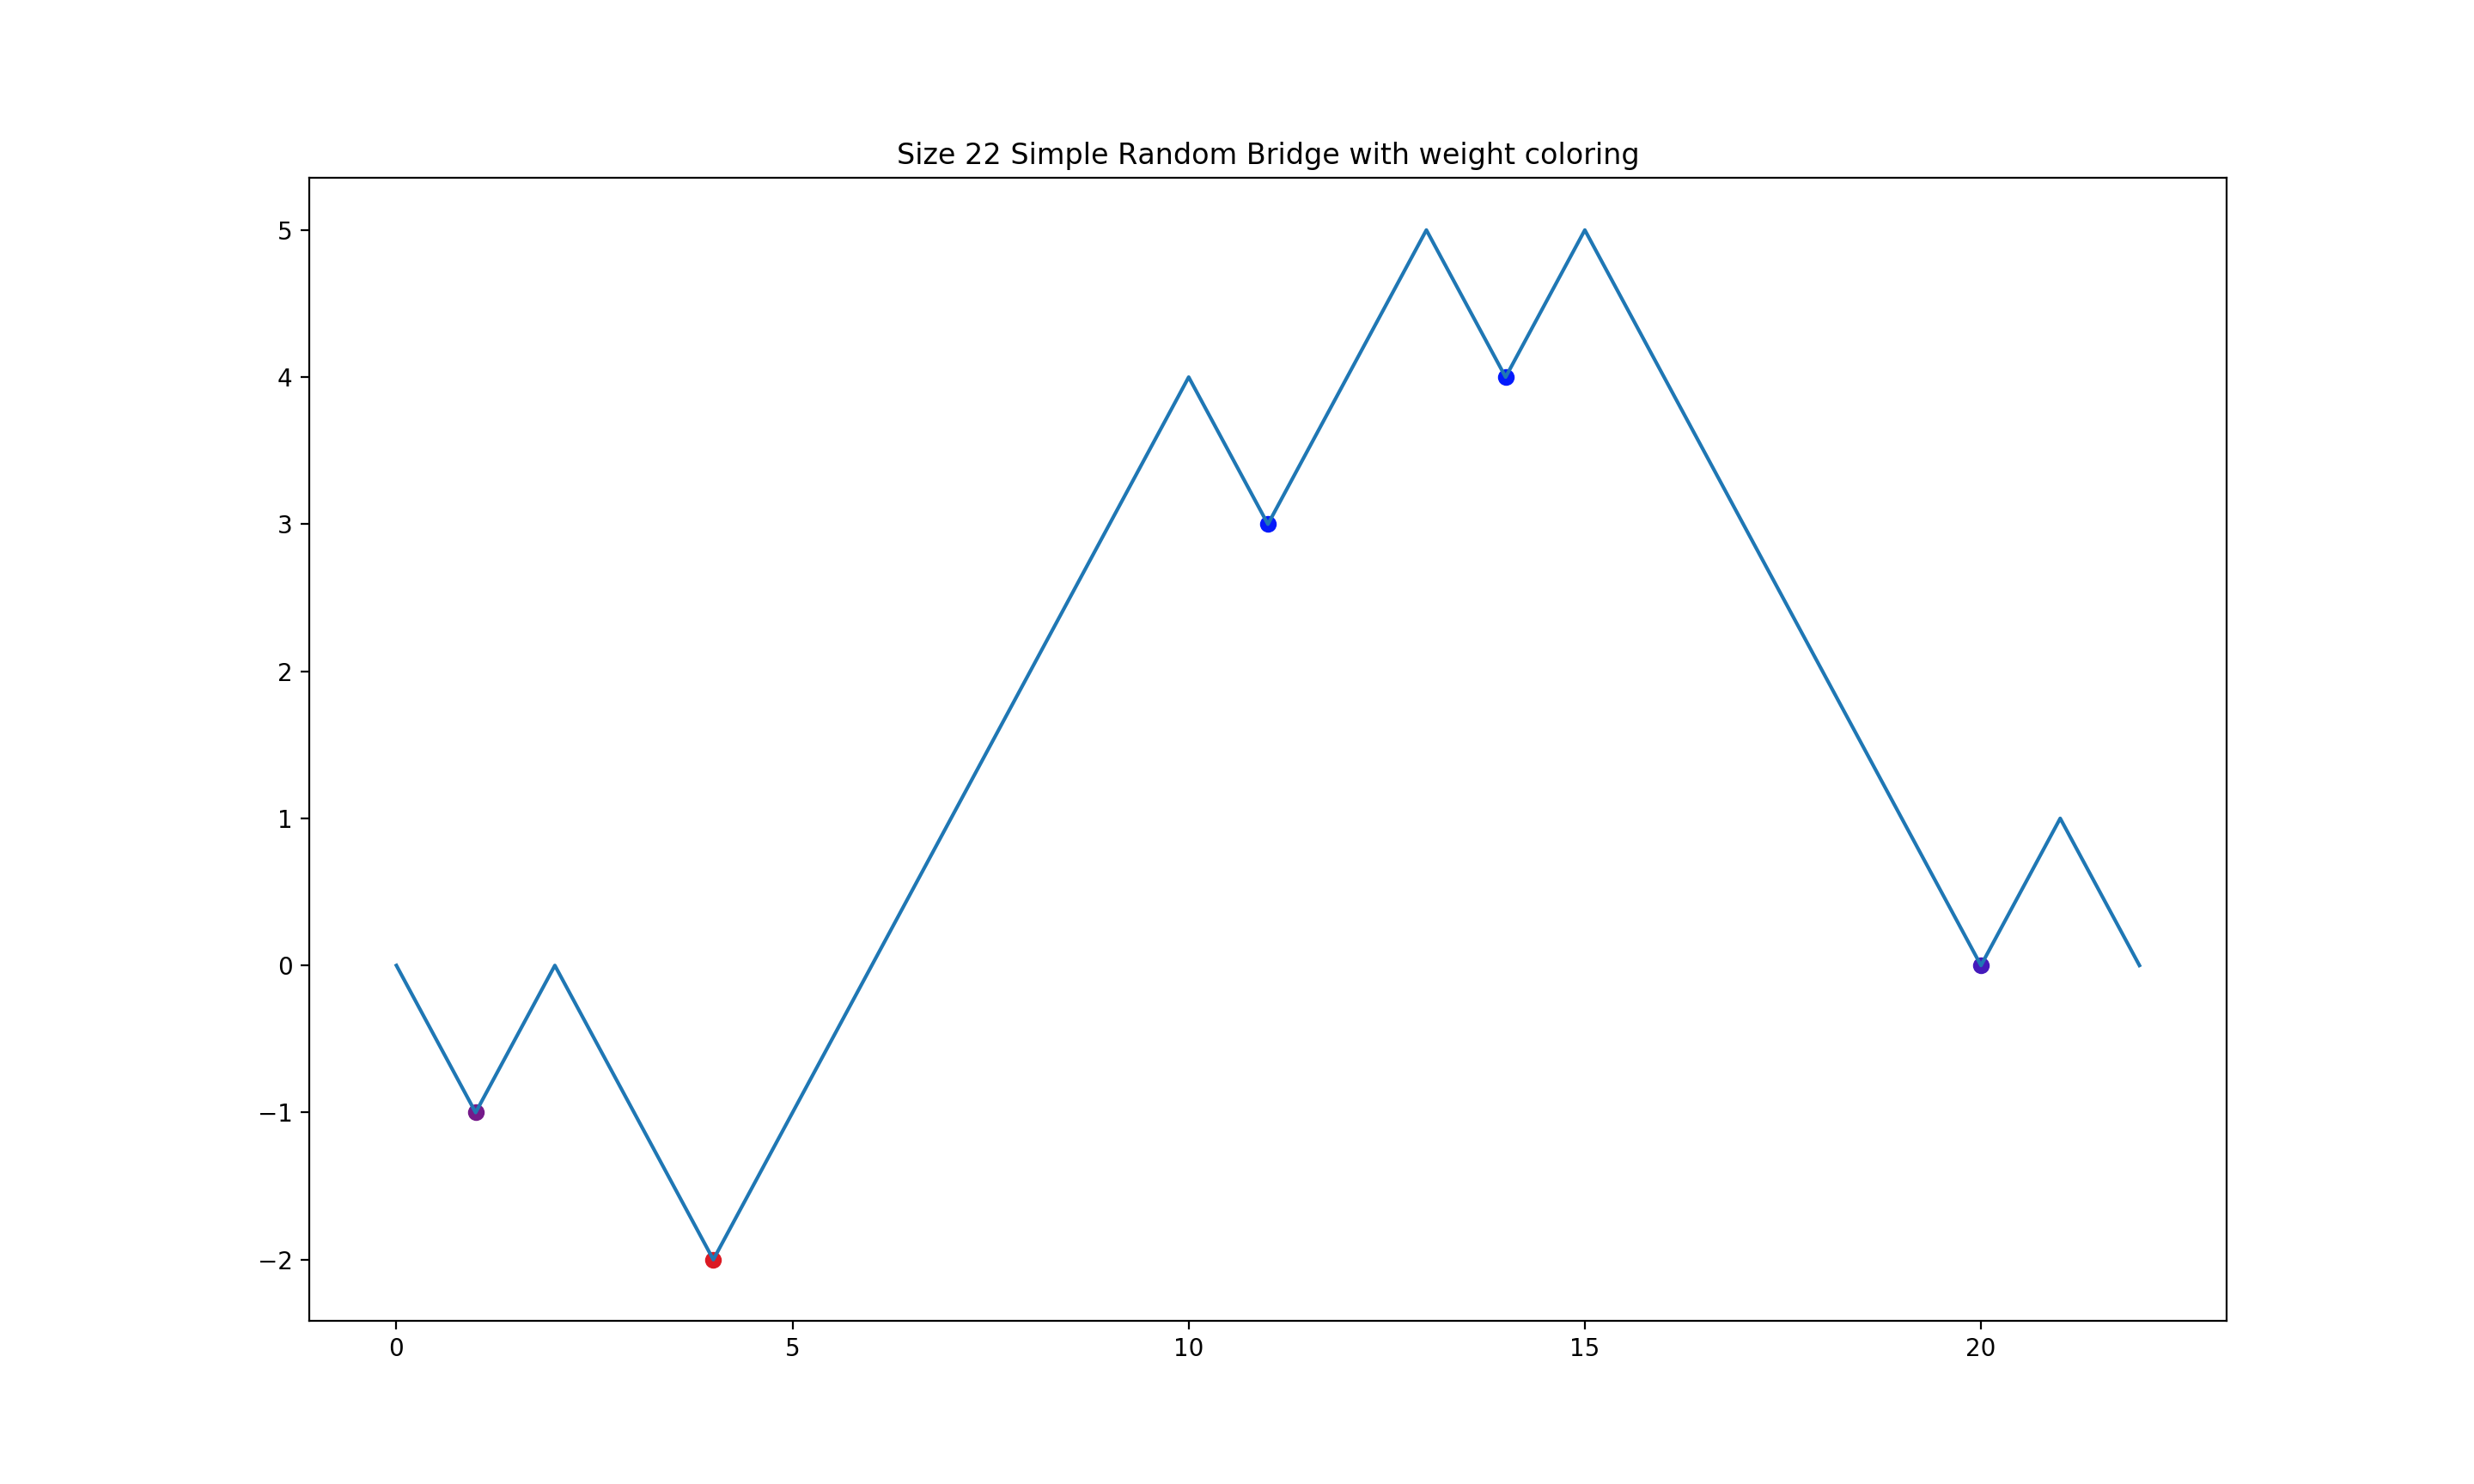
\includegraphics[width=\textwidth]{Figure_5}
\end{figure}

As a simple corollary, we arrive at a general lower bound for how likely a point is to be flipped, if it is (one of) the points the lowest in the image.

\begin{corollary} For any bridge $B$ and index $i$, if $B(i)=\min_jB(j)$ then $\Pr[i \mathrm{\,\, flips}]\geq \frac{8(N+1)}{(N+3)(N+4)}$.
\end{corollary}
\begin{proof} If we define a new Bridge $B'$ by $B'(j):=B(j+i)-B(i)$, then clearly every bridge with the Dyck word property as in the proof of Proposition 1 will once again not intersect $B'$, since by assumtion of minimality we have that $B'(j)\geq0$ uniformly. Thus,

$$|\{B_0 \,\, \mathrm{flips\,\, }i\}|\geq \frac{2}{N+4}{N+2\choose (N+2)/2}$$

and plugging this into

$$\Pr[i\,\,\mathrm{flips}]=\frac{|\{B_0 \,\, \mathrm{flips\,\, }i\}|}{|\{B_0\,\,\mathrm{of\,\,size\,\,N}\}|}$$

we are done.
\end{proof}

A general tool used in the analysis of flip probabilities is finding curves whose flip probabilities are on a known side of the starting curve, and are hopefully easier to analyse. These sorts of deformation results are very powerful, and the following conjecture would be an extremely useful variant:

\begin{conjecture}[Deformation Lemma] Let $B$ be an SRB of size $N$, $i_1$ a downed index such that $B(i_1)=\min_{j\,\,\mathrm{down}}B(j)$ and similarly $i_2$ a upped index such that $B(i_2)=\max_{j\,\,\mathrm{up}}B(j)$. Further, let

$$\tilde{B}(j)=
\begin{cases}
B(j)& j\neq i_1,i_2\\
B(j)+2 & j=i_1\\
B(j)-2 & j=i_2
\end{cases}$$

If $B(i_1)+2\leq B(i_2)-2$, then

$$\Pr[0\mathrm{\,\,flips\,\,in\,\, }\tilde{B}]\leq \Pr[0\mathrm{\,\,flips\,\,in\,\, }B]$$
\end{conjecture}

Evidence for, and reason to be skeptical about, this lemma can be found in the ``Failed Methods" section

Since $\mathbb{E}_{j\in\Z/NZ}[B(j)]=\mathbb{E}_{j\in\Z/NZ}[\tilde{B}(j)]$, this lemma can be used to create the curve that maximizes/minimizes the probability that $k$ flips for a given value of $\mathbb{E}_{j\in\Z/NZ}[B(j)]$.


\section{Interval addition}

In this section we give another notion of adding bridges $B_2$ to other bridges $B_1$, dubbed $\mathit{interval \,\,addition}$. To begin our definition, we first let

$$S=\{i\in \Z/N\Z \,\,|\,\, B_1(i)-B_2(i)=\min_j(B_1(j)-B_2(j))\}$$

be the intersection points of $B_2$ when it ``slides up" to $B_1$. We define the interval addition $\tilde{B_1}$ of $B_2$ to $B_1$ to be $B_1(i)$ if $i\not\in S$. For any subset $A\subset S$ of consecutive indicies $S$, we define $\tilde{B_1}$ on $A$ to be chosen uniformly randomly from all functions $f:A\to \Z$ such that $f(A_{i})=B_1(A_{i})$ and $f(A_{f})=B_1(A_{f})$ and $f(i+1)-f(i)=\pm1$. Here $A_i$ and $A_f$ are the initial and final indicies in $A$, which must exist since $A$ is consecutive. An example is shown in Figure 6.

\begin{figure}[h!]
\caption{Example of SRB random interval addition}
\centering
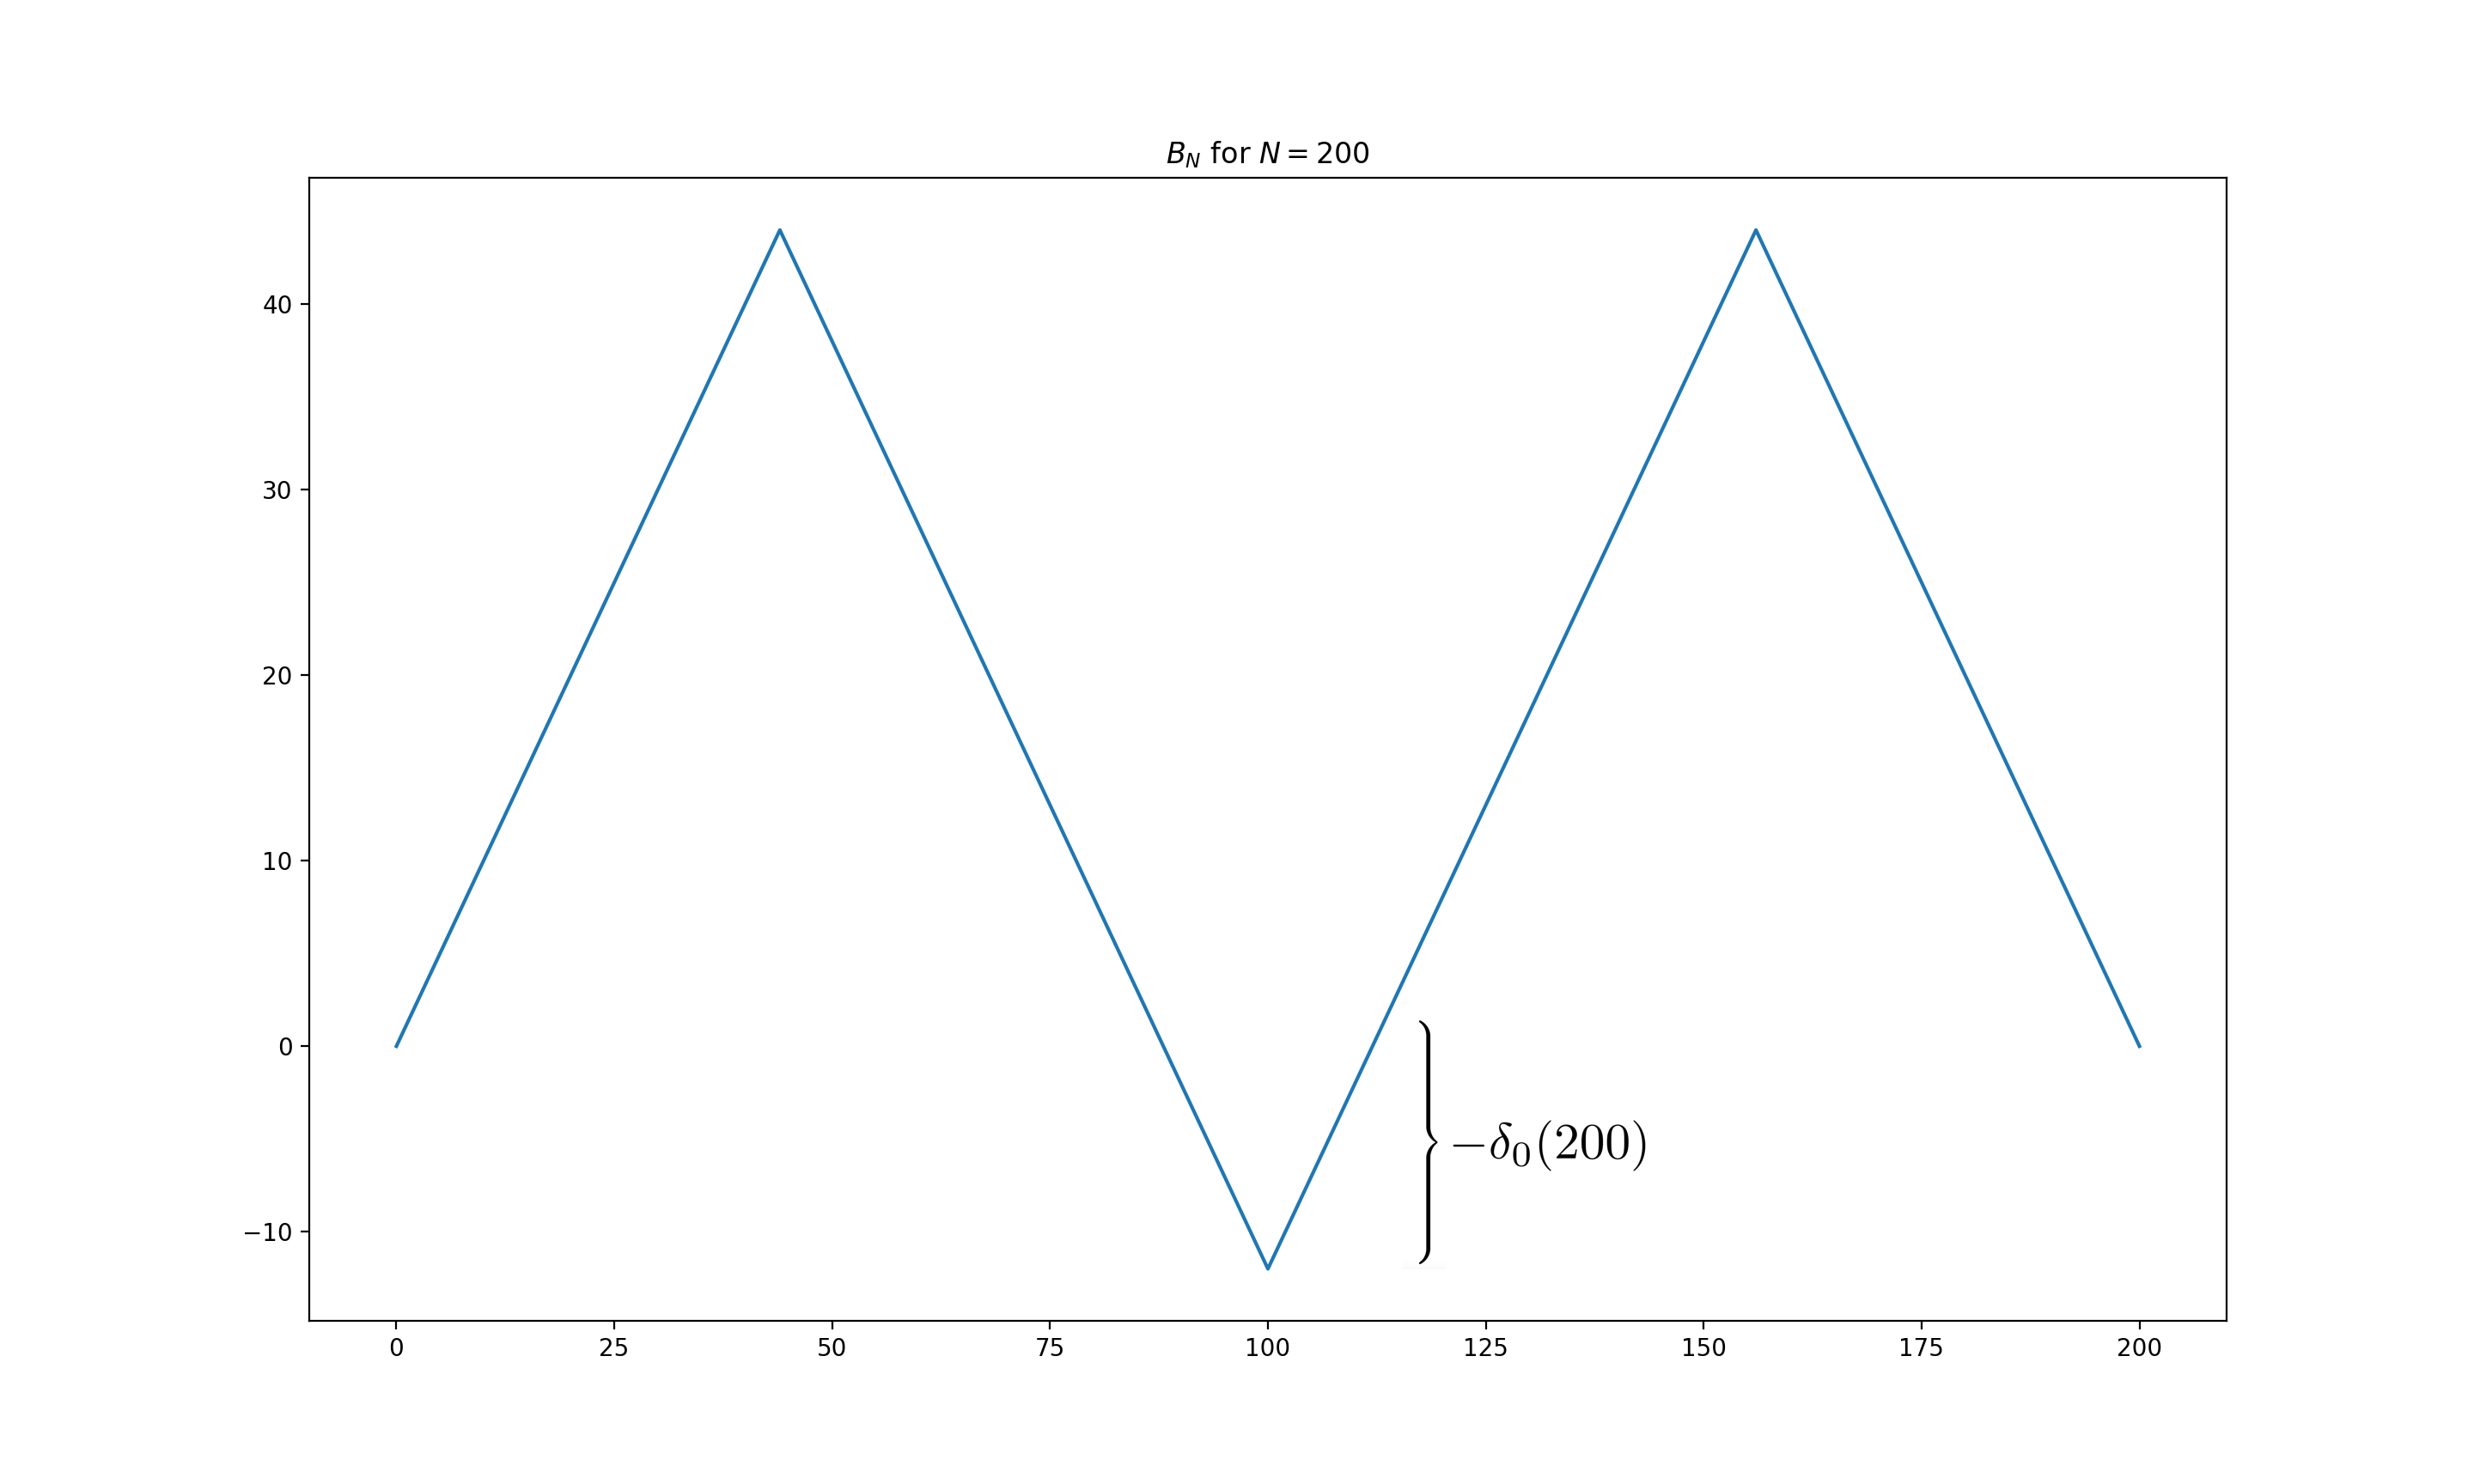
\includegraphics[width=.7\textwidth]{Figure_6}
\end{figure}


Examples of SRBs under repeated interval addition are shown in Figure 7. As can be seen in comparison with the SRBs in Figures 2/3, we see the general pattern that this sort of addition works in a much slower timeframe. As a corollary, collecting convincing data about the behavior of bridges under repeated interval addition is significantly more difficult

\begin{figure}[h!]
\caption{SRBs after repeated interval addition}
\centering
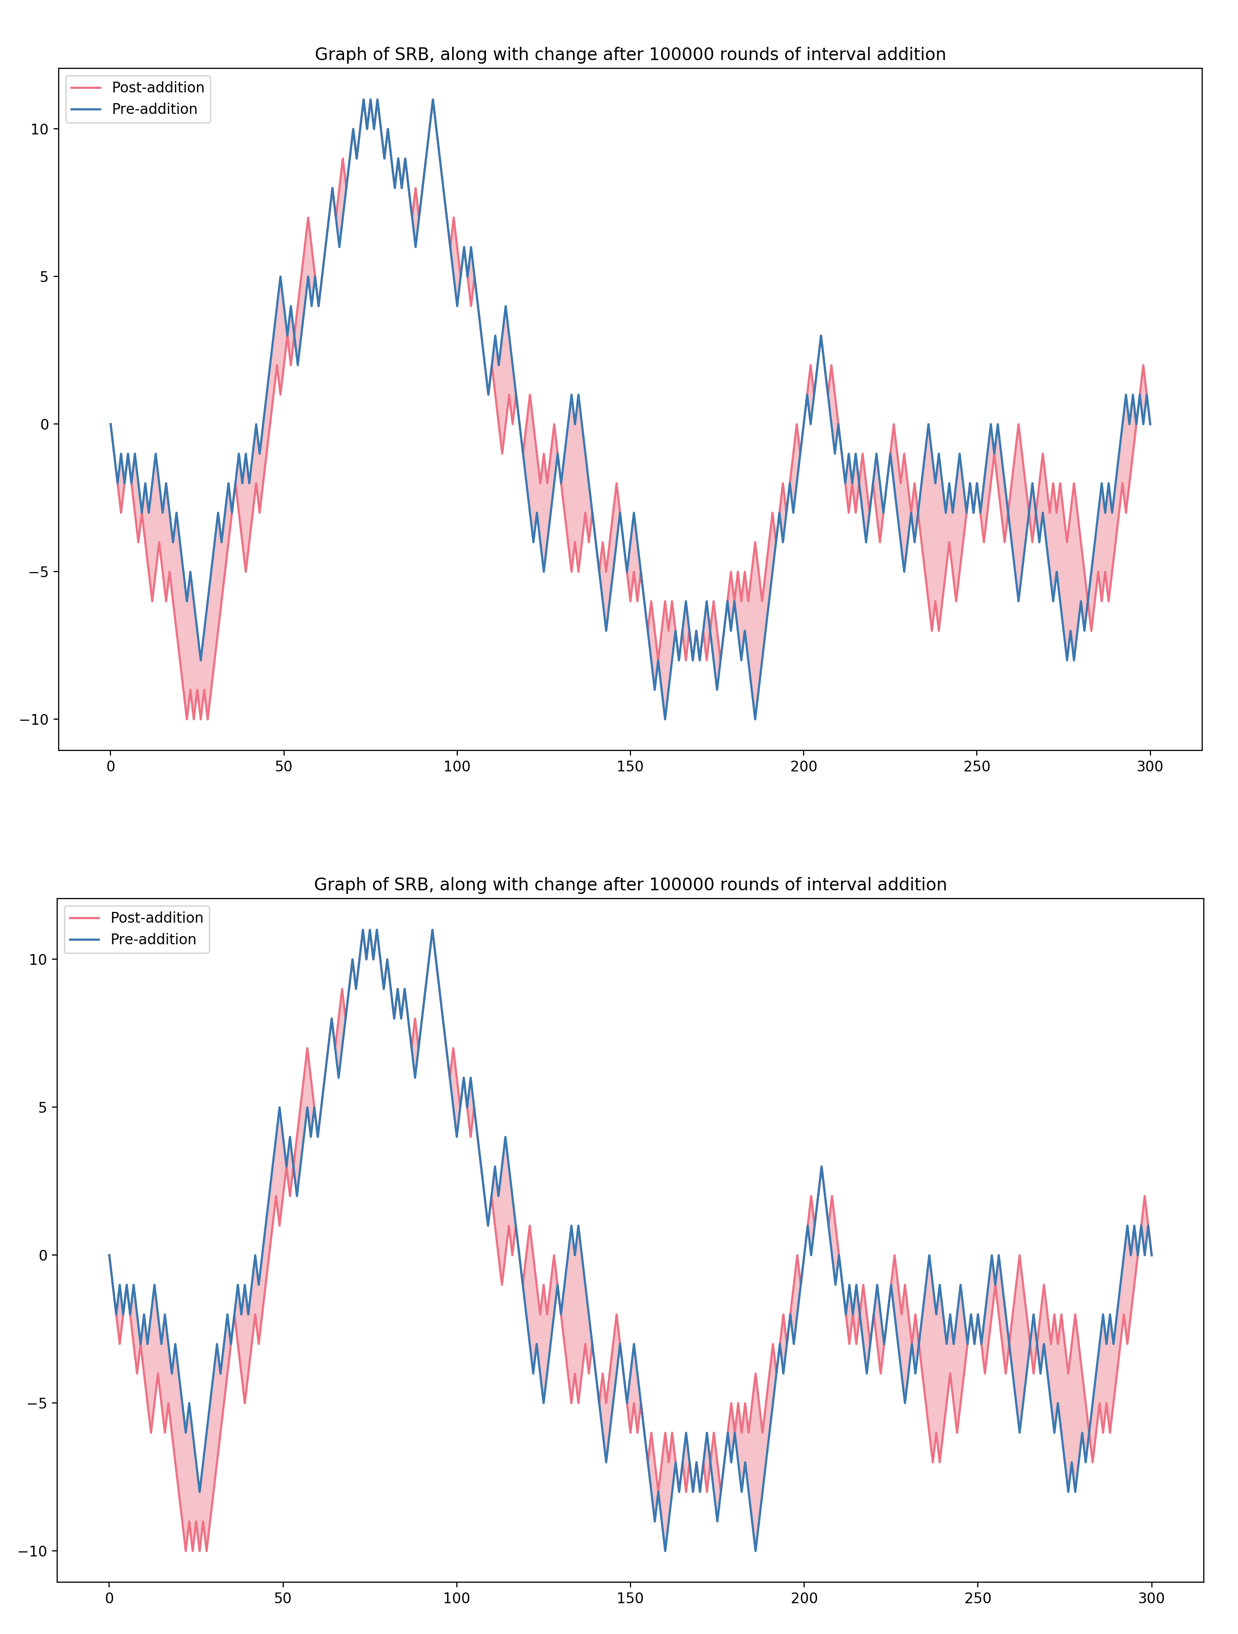
\includegraphics[width=.7\textwidth]{Figure_7}
\end{figure}

\section{Failed approaches}

In this section, we lay out directions that have been attempted in the solving of the above listed problems and why they are not effective.

The first strategy would be use Proposition 1 to show that it is likely that the minimal downed verticies are flipped, and then bound how likely all of the non-minimal downed verticies are to flip. More concretely, we can let $\delta_i:=B(i)-(\min_jB(j))$, and try to bound $\Pr[i \,\,\mathrm{flips}]$ in terms of $N$ and $\delta_i$ only. We show in the next proposition that this is not feasable

\begin{proposition} There exists a family $B_N$ of SRBs of size $N$ such that $\delta_i(N):=B_N(i)-(\min_jB_N(j))=\Omega(\sqrt{N})$ and $\Pr[i \,\, \mathrm{flips}]=\Omega(1/\sqrt{N})$.
\end{proposition}

\begin{remark}
Seeing as every bound on the probability that the minimal vertex $i$ flips will be at least on the order of $\frac{1}{\sqrt{N}}$, we see that the best that uniform bounds on $\Pr[i \,\, \mathrm{flips}]$ will do is prove that under repeated addition $\E[\max_i|B(i)|]=O(\sqrt{N})$  which also follows directly from the Central Limit Theorem.
\end{remark}

\begin{proof}[Proof of Proposition 2] Throughout this proof we assume that $N\equiv0\,\,\mathrm{mod}(4)$, since the case $N\equiv 2\,\,\mathrm{mod}(4)$ is done similarly. Let $B_N$ be a family of curves with

$$\delta_0(N)=\lfloor \sqrt{N}\rfloor - (\lfloor \sqrt{N}\rfloor\,\,\mathrm{mod}(2))$$

and piecewise definition

\begin{equation*}
B_N(j)=
\begin{cases}
j & 0\leq j < \frac{N}{4}-\frac{\delta_0(N)}{2}\\
\frac{N}{2}-\delta_0(N)-j & \frac{N}{4}-\frac{\delta_0(N)}{2}\leq j \leq \frac{N}{2}\\
B_N(j)=B_N(N-j) & \frac{N}{2}<j<N
\end{cases}
\end{equation*}


This SRB is shown in Figure 8.

\begin{figure}[h!]
\caption{An example of the SRBs $B_N$}
\centering
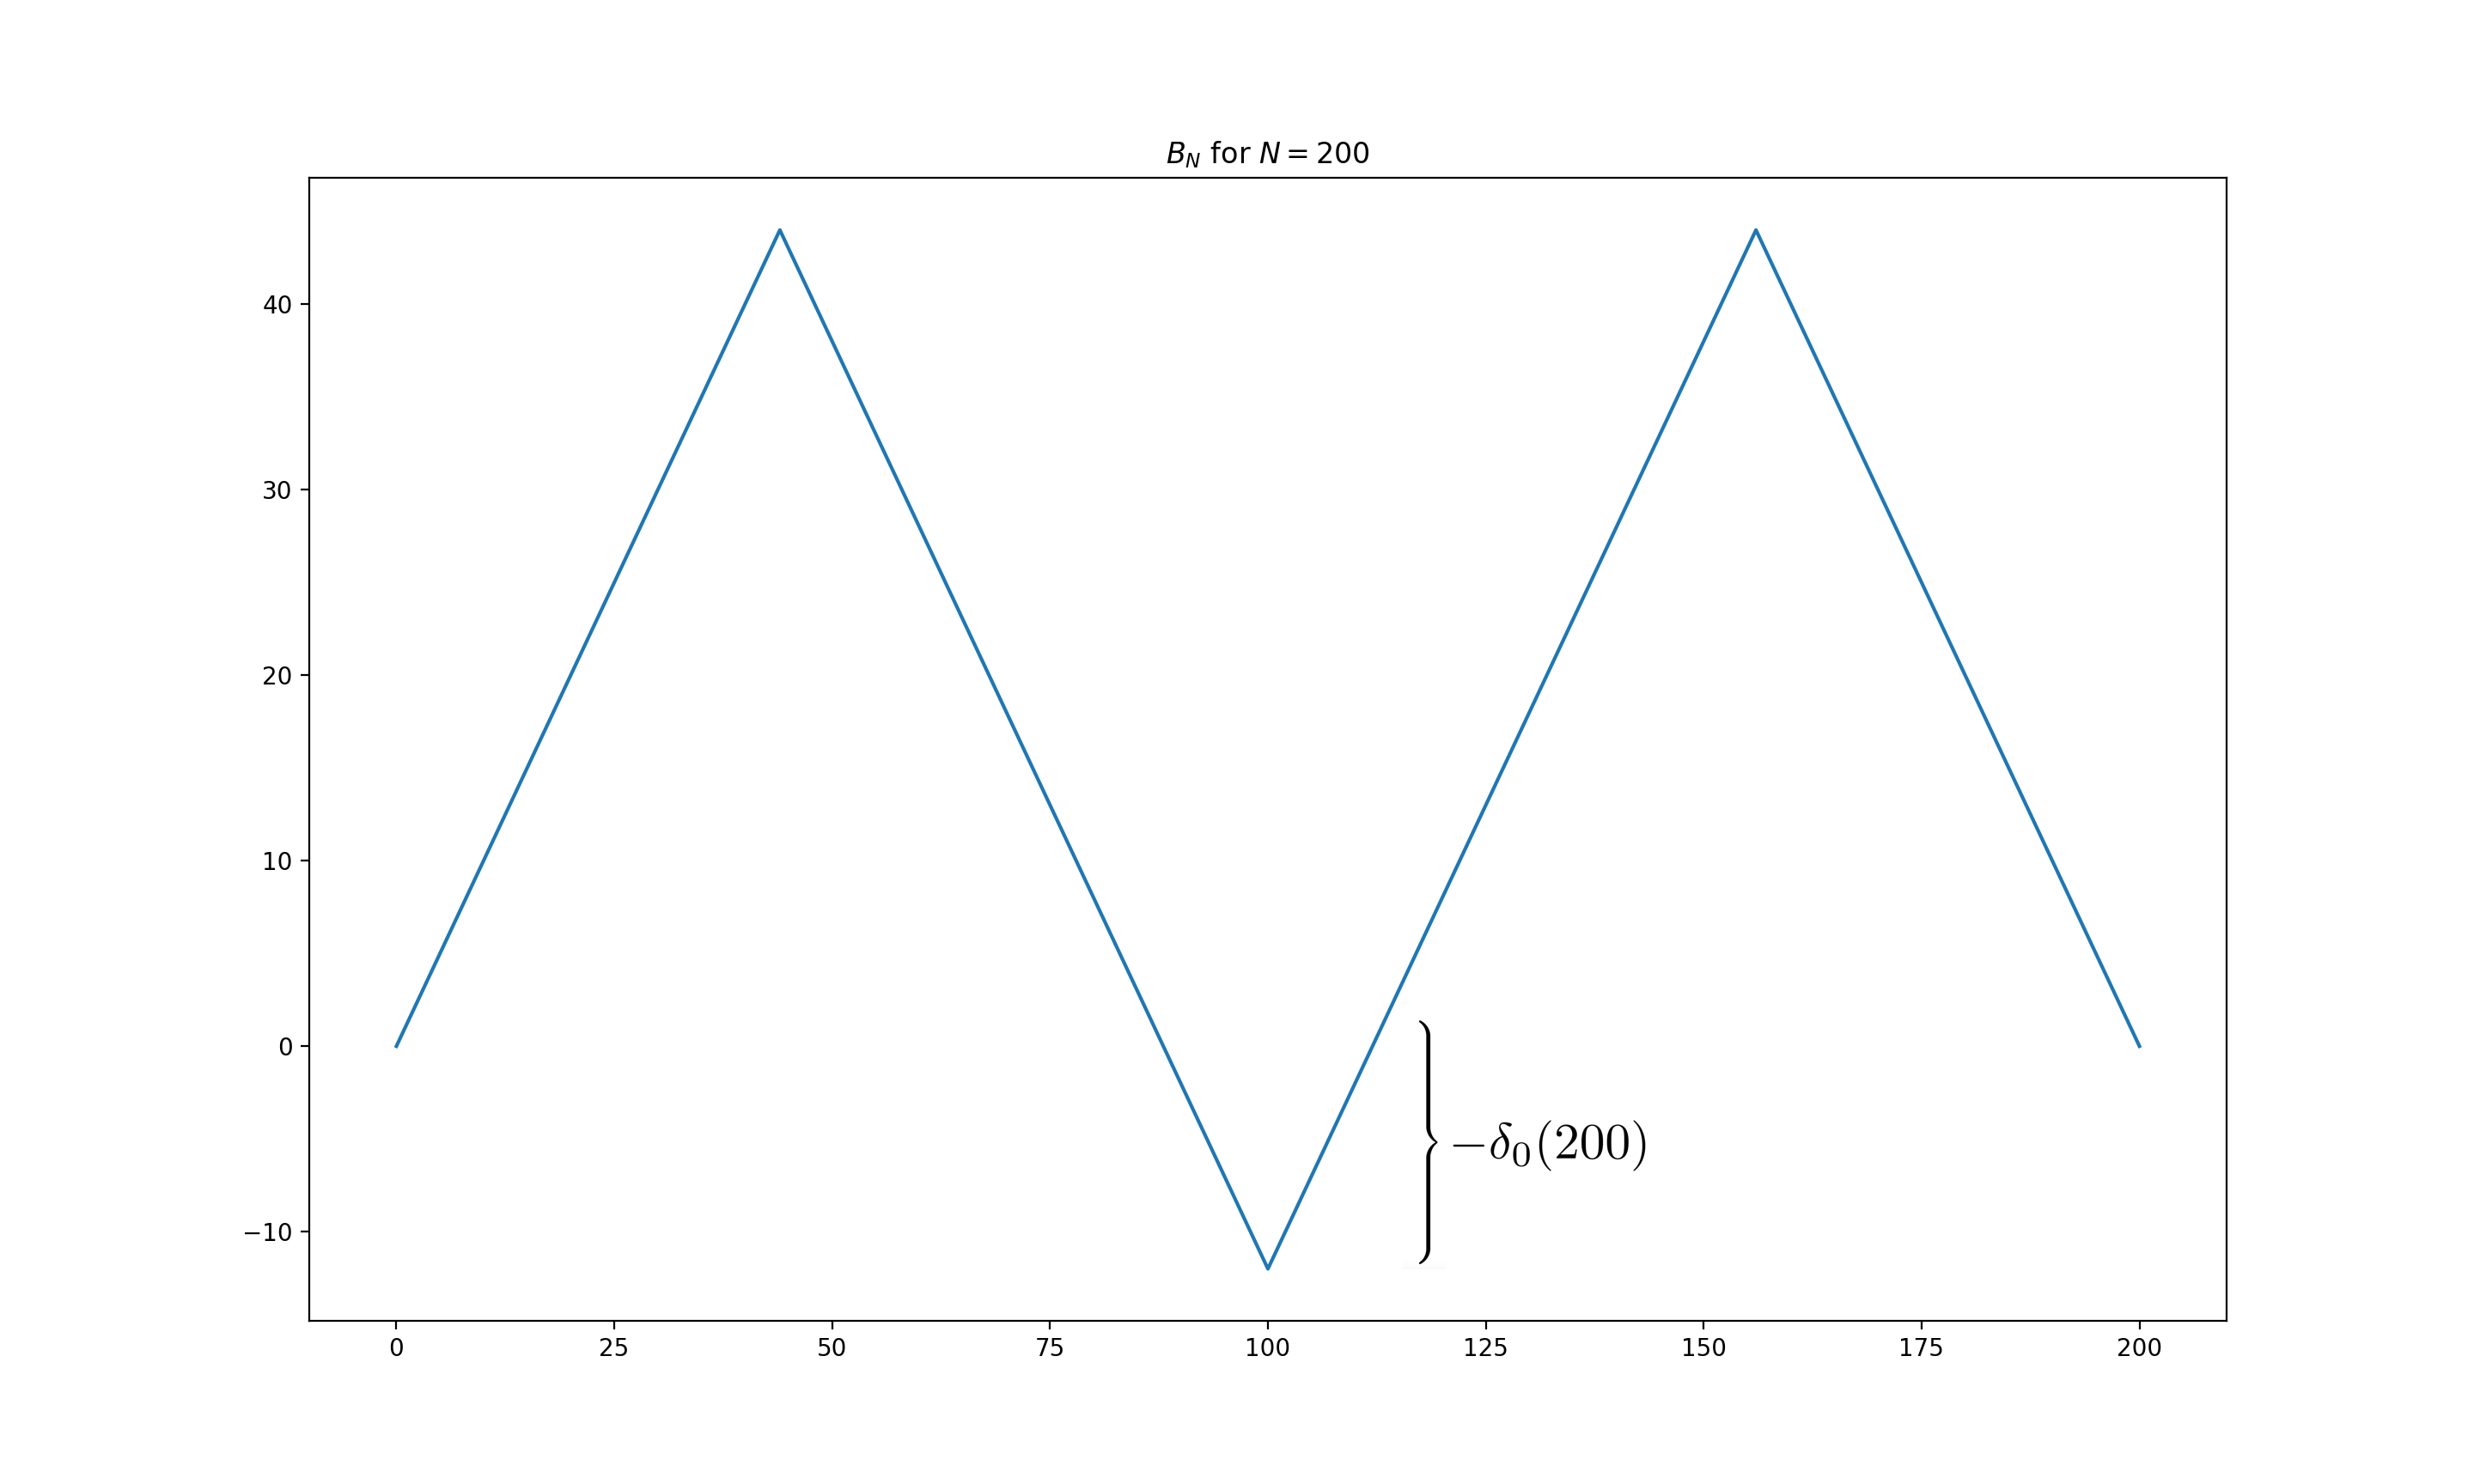
\includegraphics[width=\textwidth]{Figure_8}
\end{figure}

Using the same trick as in the proof of Proposition 1, we get that

\begin{equation*}
\Pr[0\,\,\mathrm{flips}]=\frac{1}{{N \choose N/2}}|\{B_0 \,\, \mathrm{flips\,\, }0\}|
\end{equation*}

By the definition of $B_N$ we know that the bridges $B_0$ that stay below $B_N$ are exactly those that stay below $B_N$ at $i=N/2$. Seeing as those SRBs that touch $B_N$ exactly at $B(N/2)=-\delta_0(200)$ fit this criteria, we get that there are at least

$${N/2 \choose N/4-\frac{\delta_0(N)}{2}}^2$$

bridges that satisfy the criteria. By an explicit calculation this means that

\begin{equation*}
\Pr[0\,\,\mathrm{flips}]\geq \frac{{N/2 \choose N/4}^2}{{N \choose N/2}\left(1-\frac{2m}{N}\right)^{2}} \prod_{j=1}^{\frac{m}{2}}\left(\frac{1-\frac{4j}{N}}{1+\frac{4j}{N}}\right)^{2}
\end{equation*}

By Strirlings approximation (see, for example, \cite{eger2014stirling}) we have that

$$\frac{{N/2 \choose N/4}^2}{{N \choose N/2}}\sim \frac{4}{\sqrt{2\pi N}}$$

and since $m/2<\sqrt{N}/2$ we have that

\begin{align*}
\prod_{j=1}^{\frac{m}{2}}\left(\frac{1-\frac{4j}{N}}{1+\frac{4j}{N}}\right)&=\exp\left(\sum_{j=1}^{m/2}\ln\left(\frac{1-\frac{4j}{N}}{1+\frac{4j}{N}}\right)\right)\\
&\geq \exp\left(\sum_{j=1}^{\sqrt{N}/2}\ln\left(\frac{1-\frac{2}{\sqrt{N}}}{1+\frac{2}{\sqrt{N}}}\right)\right)\\
&=\Omega\left( \exp\left(\sum_{j=1}^{\sqrt{N}/2}\frac{1}{\sqrt{N}}\right)\right)\\
&=\Omega(1)
\end{align*}


which completes the proof.
\end{proof}

As of now, the strategy of deformations (as seen in Conjecture 2) has not been successful. The most natural way to state the deformation conjecture would be to remove the condition $B(i_1)=\mathrm{min}_{j\,\,\mathrm{down}}B(j)$ and $B(i_2)=\mathrm{nax}_{j\,\,\mathrm{up}}B(j)$. Flipping a low vertex up and a high vertex down should always result in the increase of probability 0 flips. This conjecture was beleived for a long time, but here is strong counterexample:

\begin{figure}[h!]
\caption{A counterexample to the first deformation conjecture}
\centering
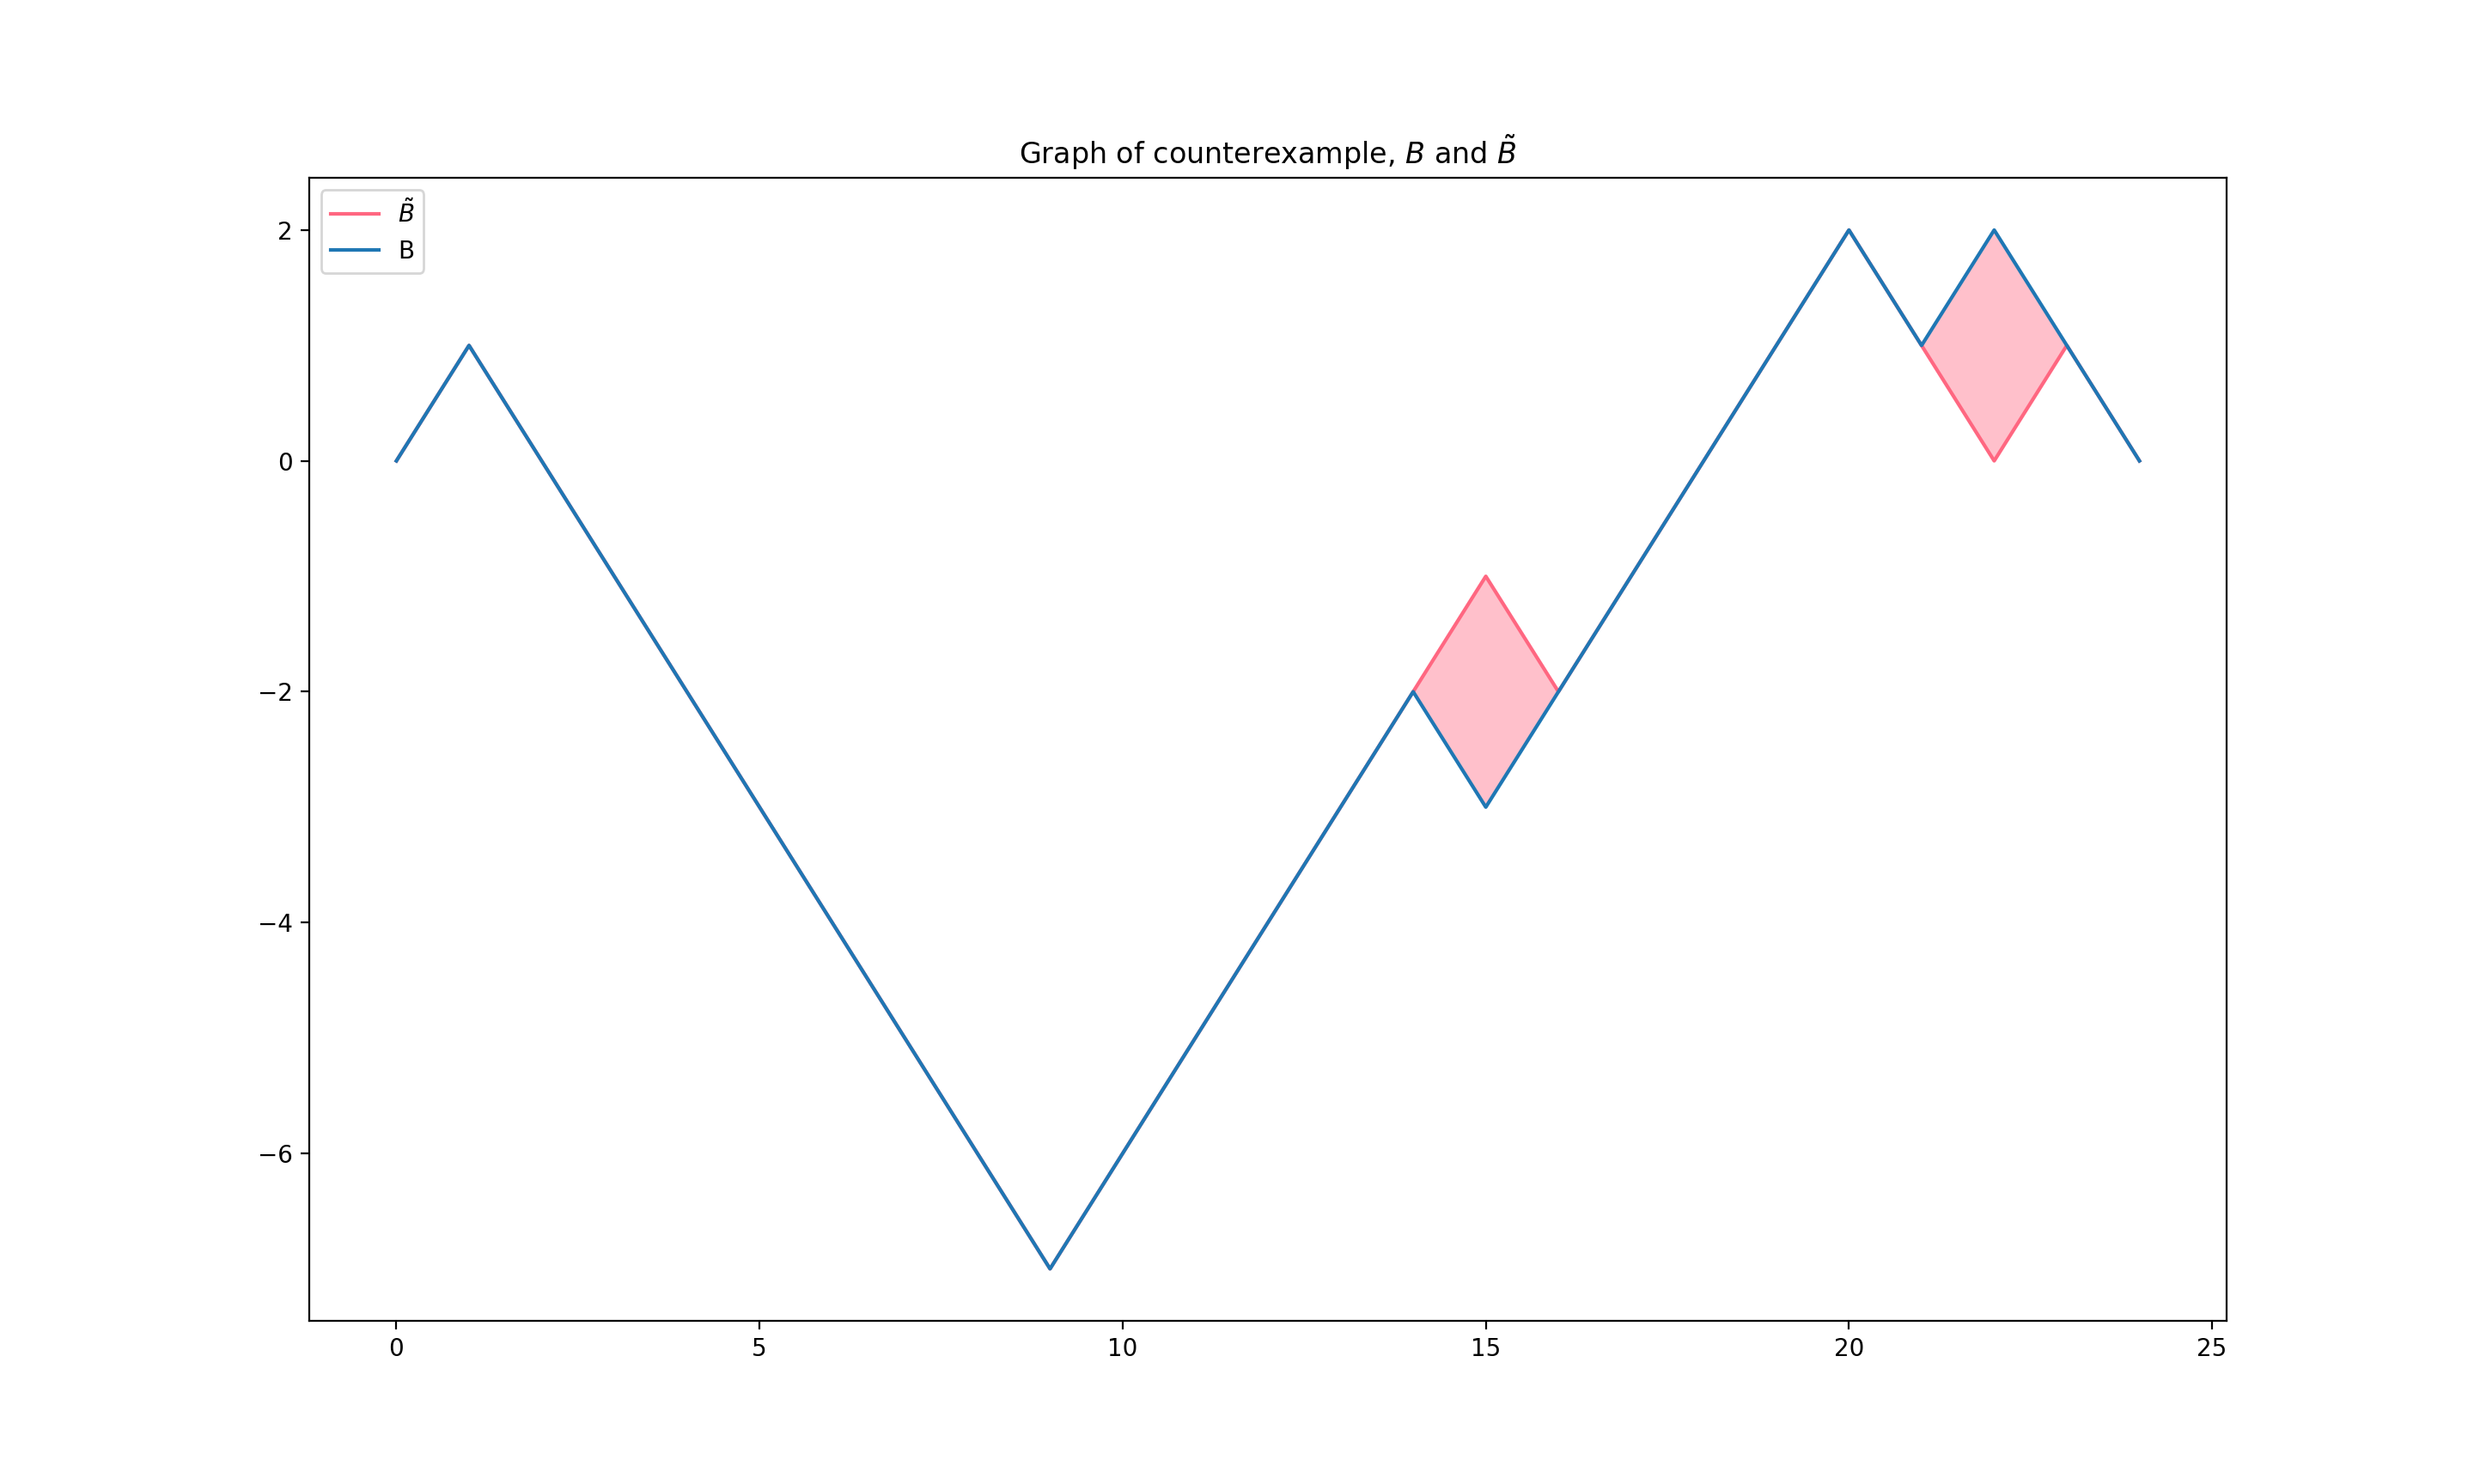
\includegraphics[width=\textwidth]{Figure_9}
\end{figure}

Here, we have

$$\Pr[0\,\,\mathrm{flips\,\,in\,\, B}]\approx 0.004263$$

and

$$\Pr[0\,\,\mathrm{flips\,\,in\,\, \tilde{B}}]\approx 0.004271$$

In particular, $\Pr[0\,\,\mathrm{flips\,\,in\,\, B}]<\Pr[0\,\,\mathrm{flips\,\,in\,\, \tilde{B}}]$


\bibliographystyle{plain}
\bibliography{ref}


\end{document}

